\chapter{Project}
At the end of the internship, we were assigned a task to develop an application using Flutter. I made a to-do List application, with the following features:\\
\begin{itemize}
\item Login and Signup with Firestore authentication as backend
\item Two user friendly themes (Light theme and dark theme)
\item Minimalistic Design
\item Data synchronisation on Firestore firebase cloud
\end{itemize}
\hfill
\newpage

\subsection{Login and Signup with Firestore Authentication}

\begin{figure}
  \begin{center}
  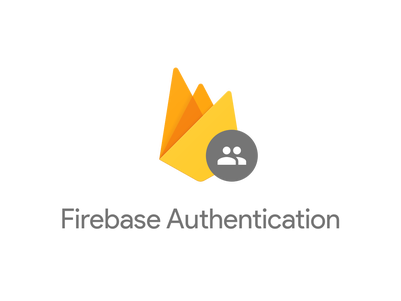
\includegraphics[height=80mm]{Images & Logos/CH_08_FirebaseAuth.png}
  \end{center}
  \caption{Firebase Authentication Logo}
\end{figure}

In the present era, user authentication is one of the most important requirements for Android apps. It is essential to authenticate users, and it is much harder if we have to write all this code on our own. This is done very easily with the help of Firebase.
\begin{itemize}
\item Being able to authenticate our users securely, it offers a customized experience to them based on their interests and preferences.
\item We can ensure that they have no problems accessing their private data while using our app from multiple devices.
\item Firebase Authentication provides all the server-side stuff for authenticating the user. Firebase Authentication becomes easy with SDK. It makes API easy to use.
\item Firebase Authentication also provides some user interface libraries which enable screens for us when we are logging it.
\item Firebase authentication supports authentication using a password, phone numbers, popular identity provider like Google, Facebook, and Twitter, etc.
\item We can sign in users to our app by using the FirebaseUI.
\item It handles the UI flows for signing in user with an email address and password, phone numbers, and popular providers, including Google sign-In and Facebook Login
\item It can also handle cases like account recovery.
\item It is not required to design a UI since it is already provided for us. It means we don't have to write the activities.
\item We can also sign-in users using the Firebase Authentication SDK to integrate one or several sign-in methods into our app manually.

\end{itemize}
\newpage
\section{Two user friendly themes}
In the To-Do List app i created,  i had two themes i.e. dark mode and light mode for the users to have good user experience.

\subsection{Light Mode}
\begin{itemize}
\item White background
\item Grey Buttons (HexCode : \#EAEAEA)
\item Black icons
\item Green Update and Complete task button
\end{itemize}
%\begin{figure}[h]
%  \begin{center}
%   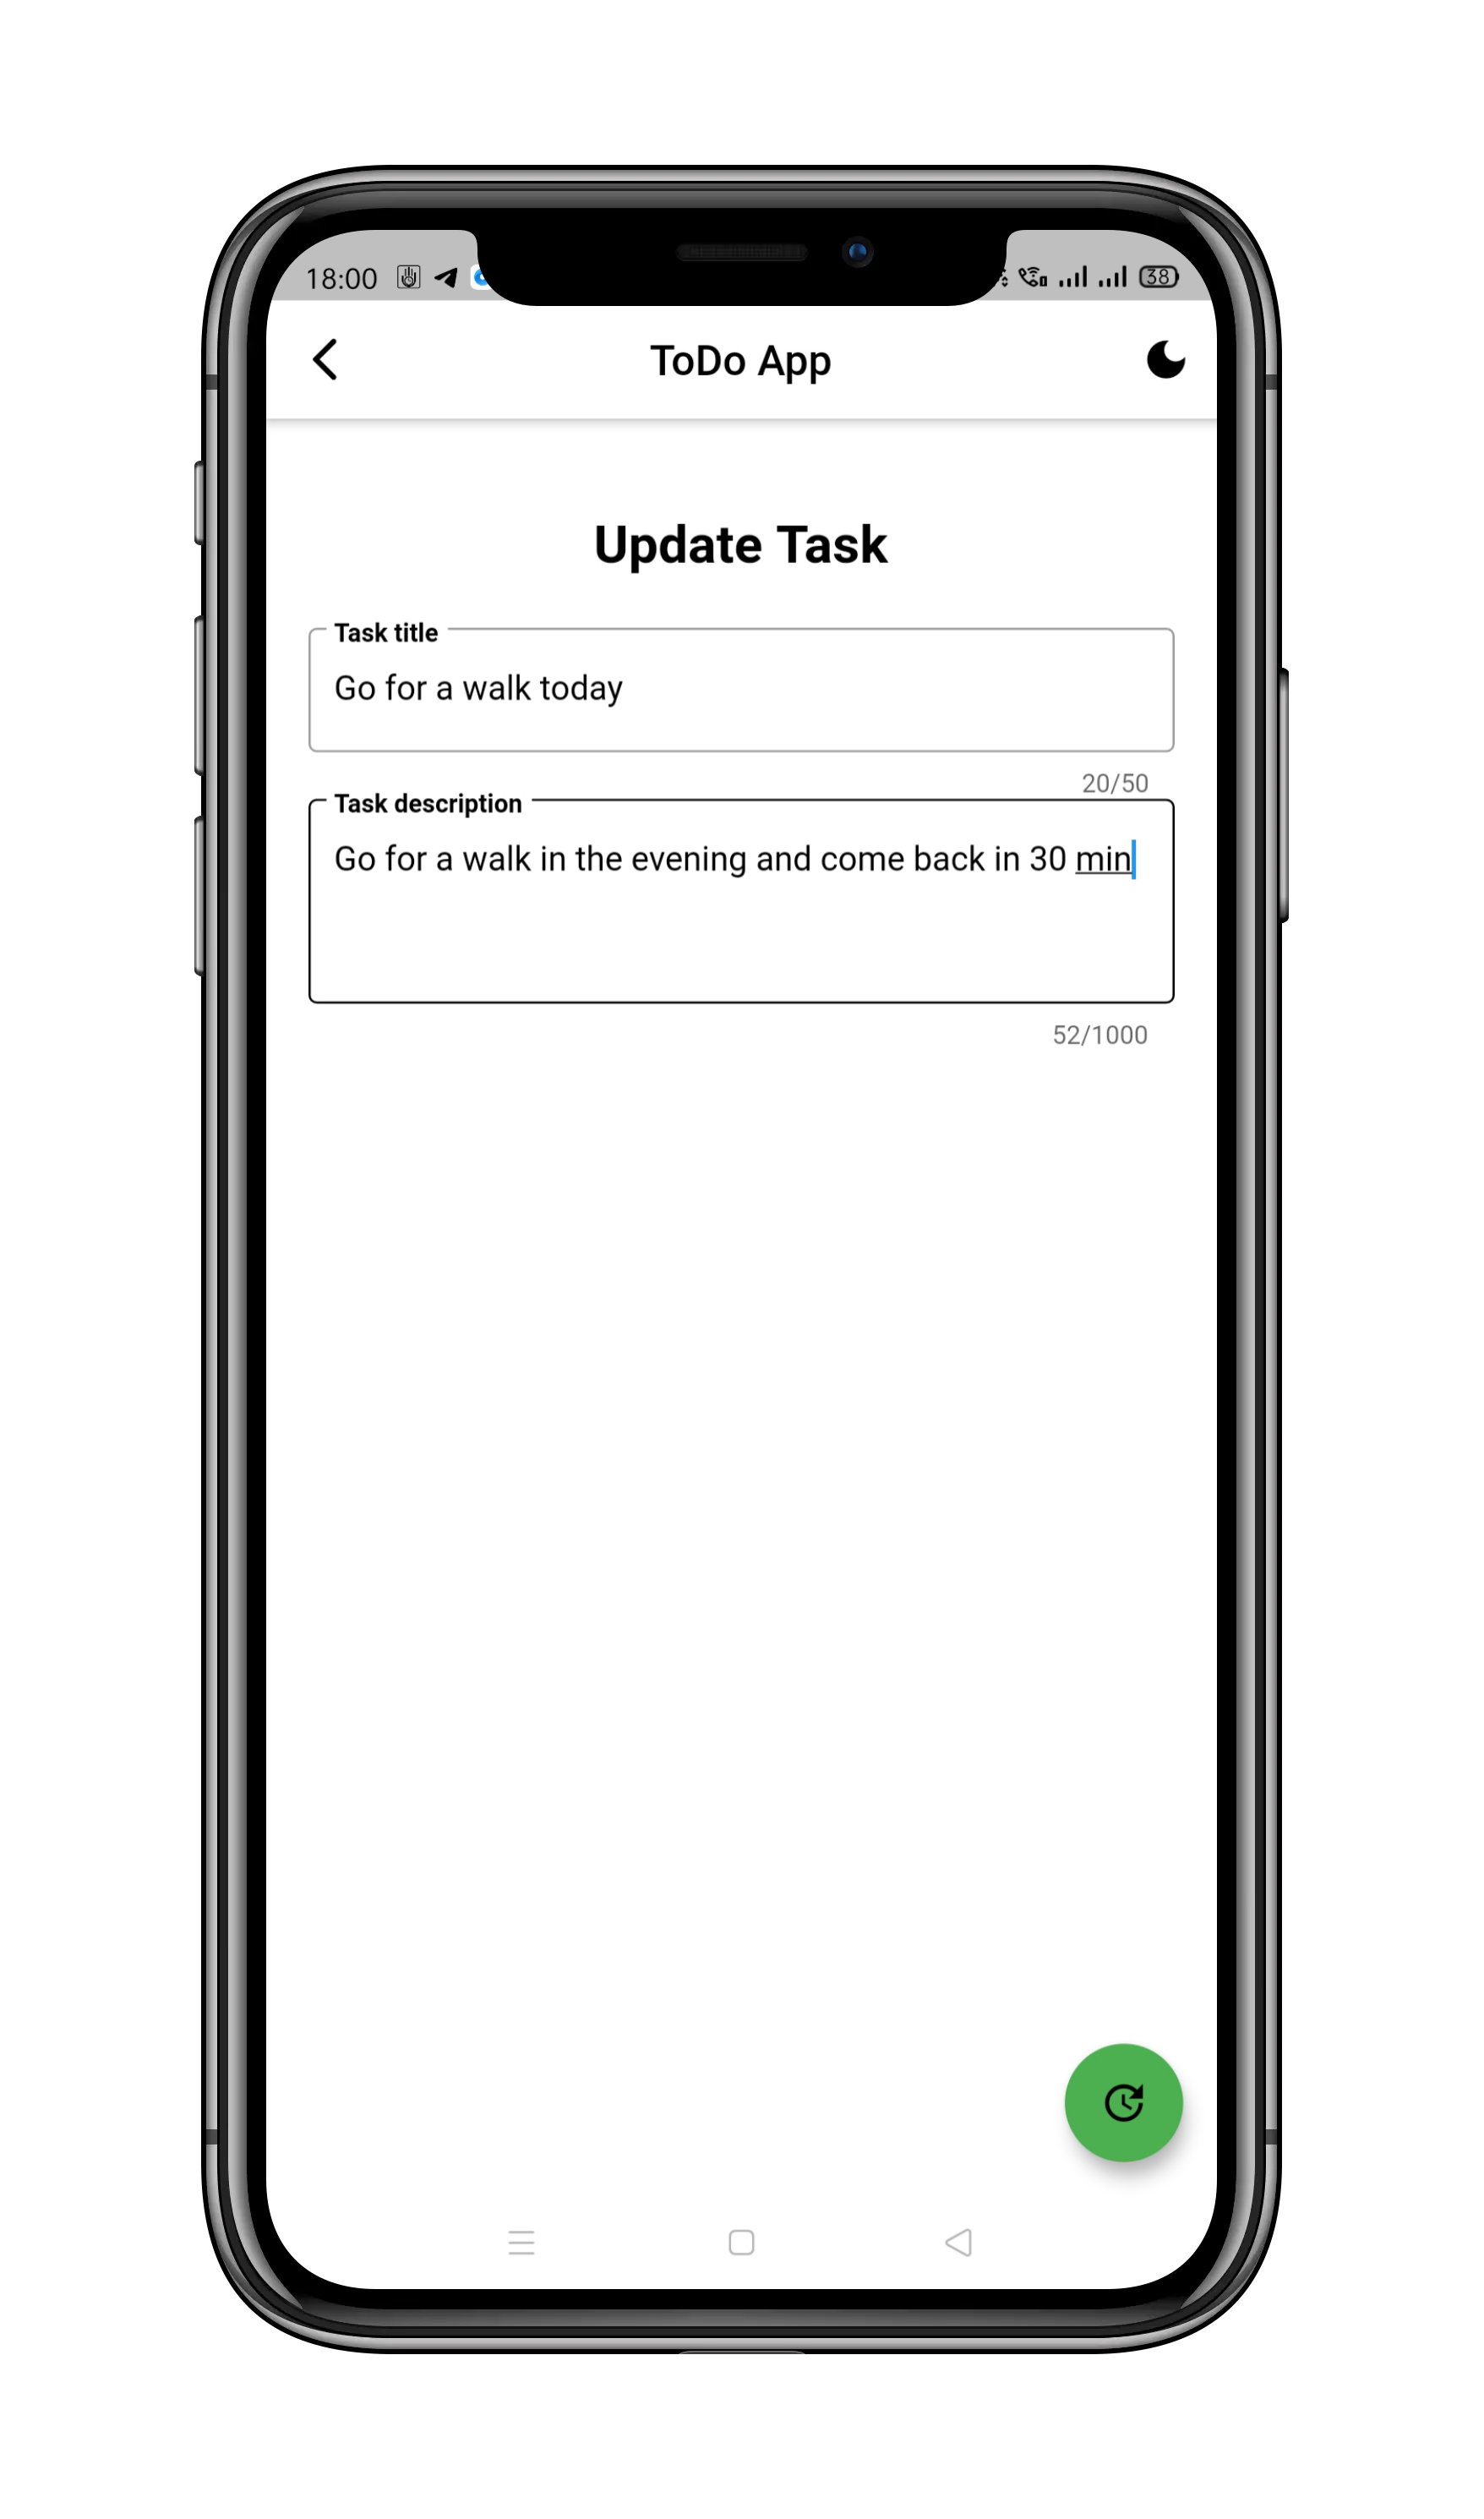
\includegraphics[height=90mm]{Images & Logos/theme/CH_08_Light_5.png}
%  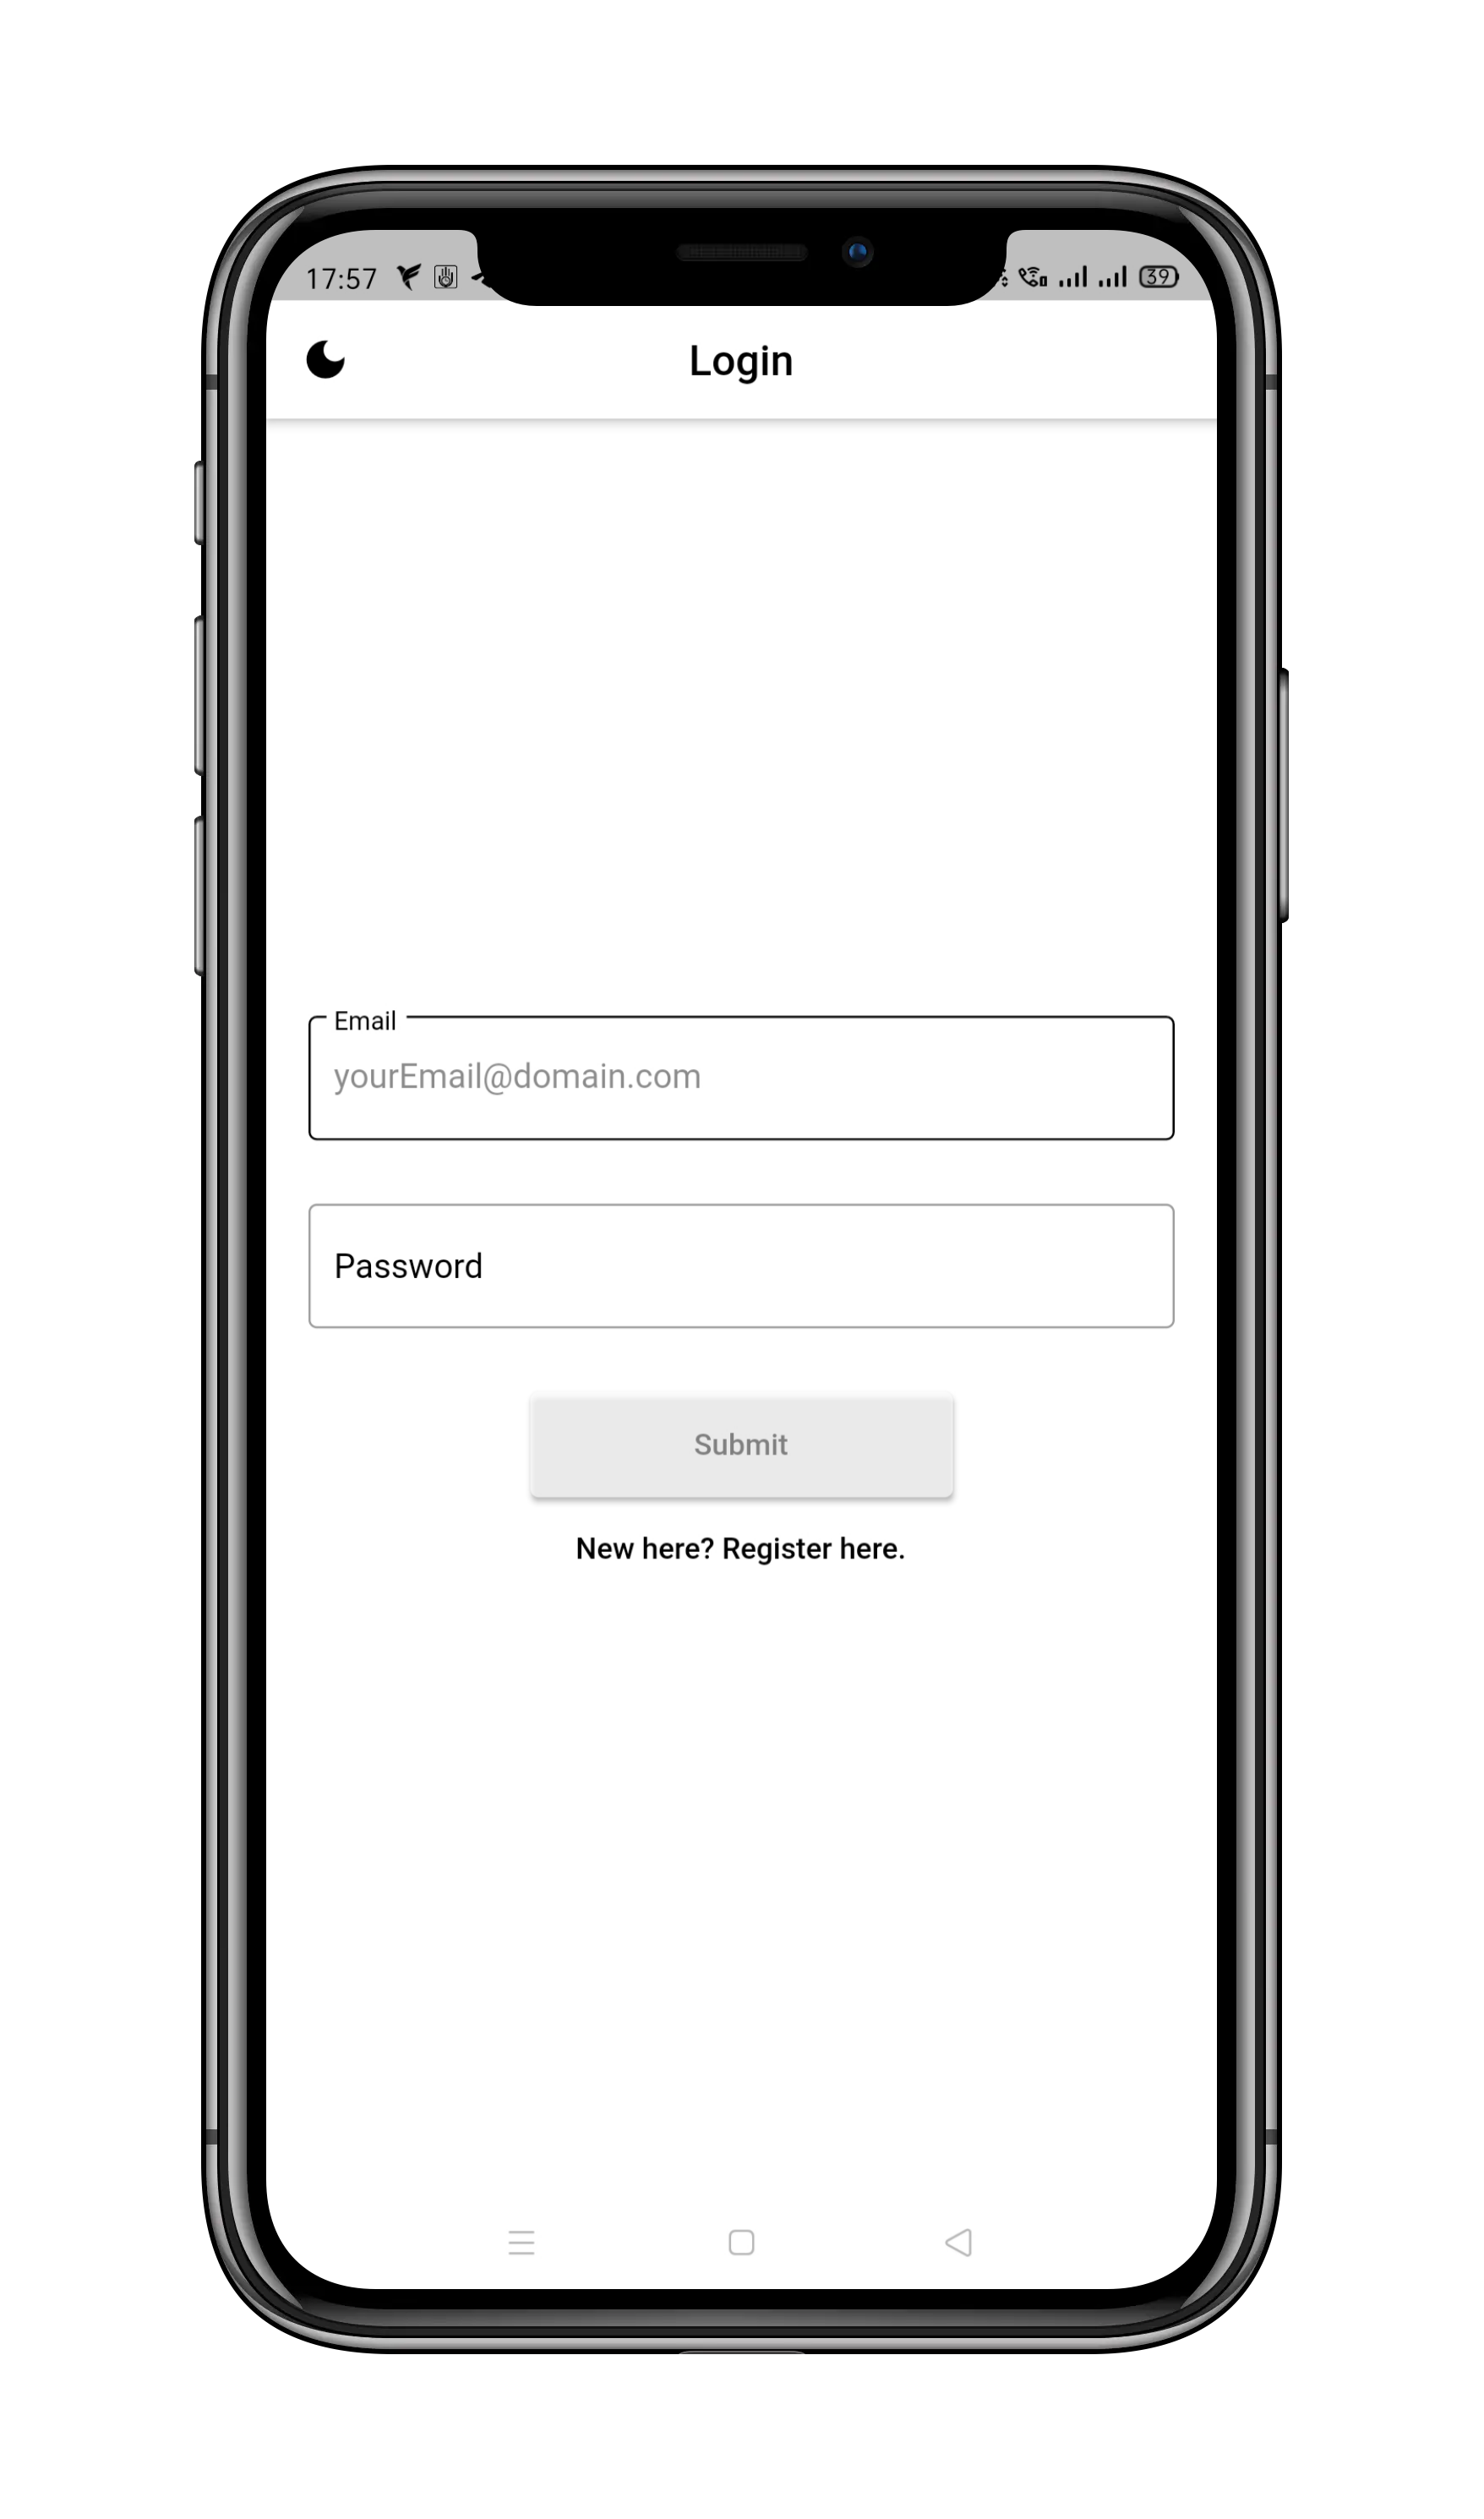
\includegraphics[height=70mm]{Images & Logos/theme/CH_08_Light_1.png}\\
%  \end{center}
%  \caption{Light Mode}
%\end{figure}  
\begin{figure}
\centering
\begin{minipage}{.5\textwidth}
  \centering
   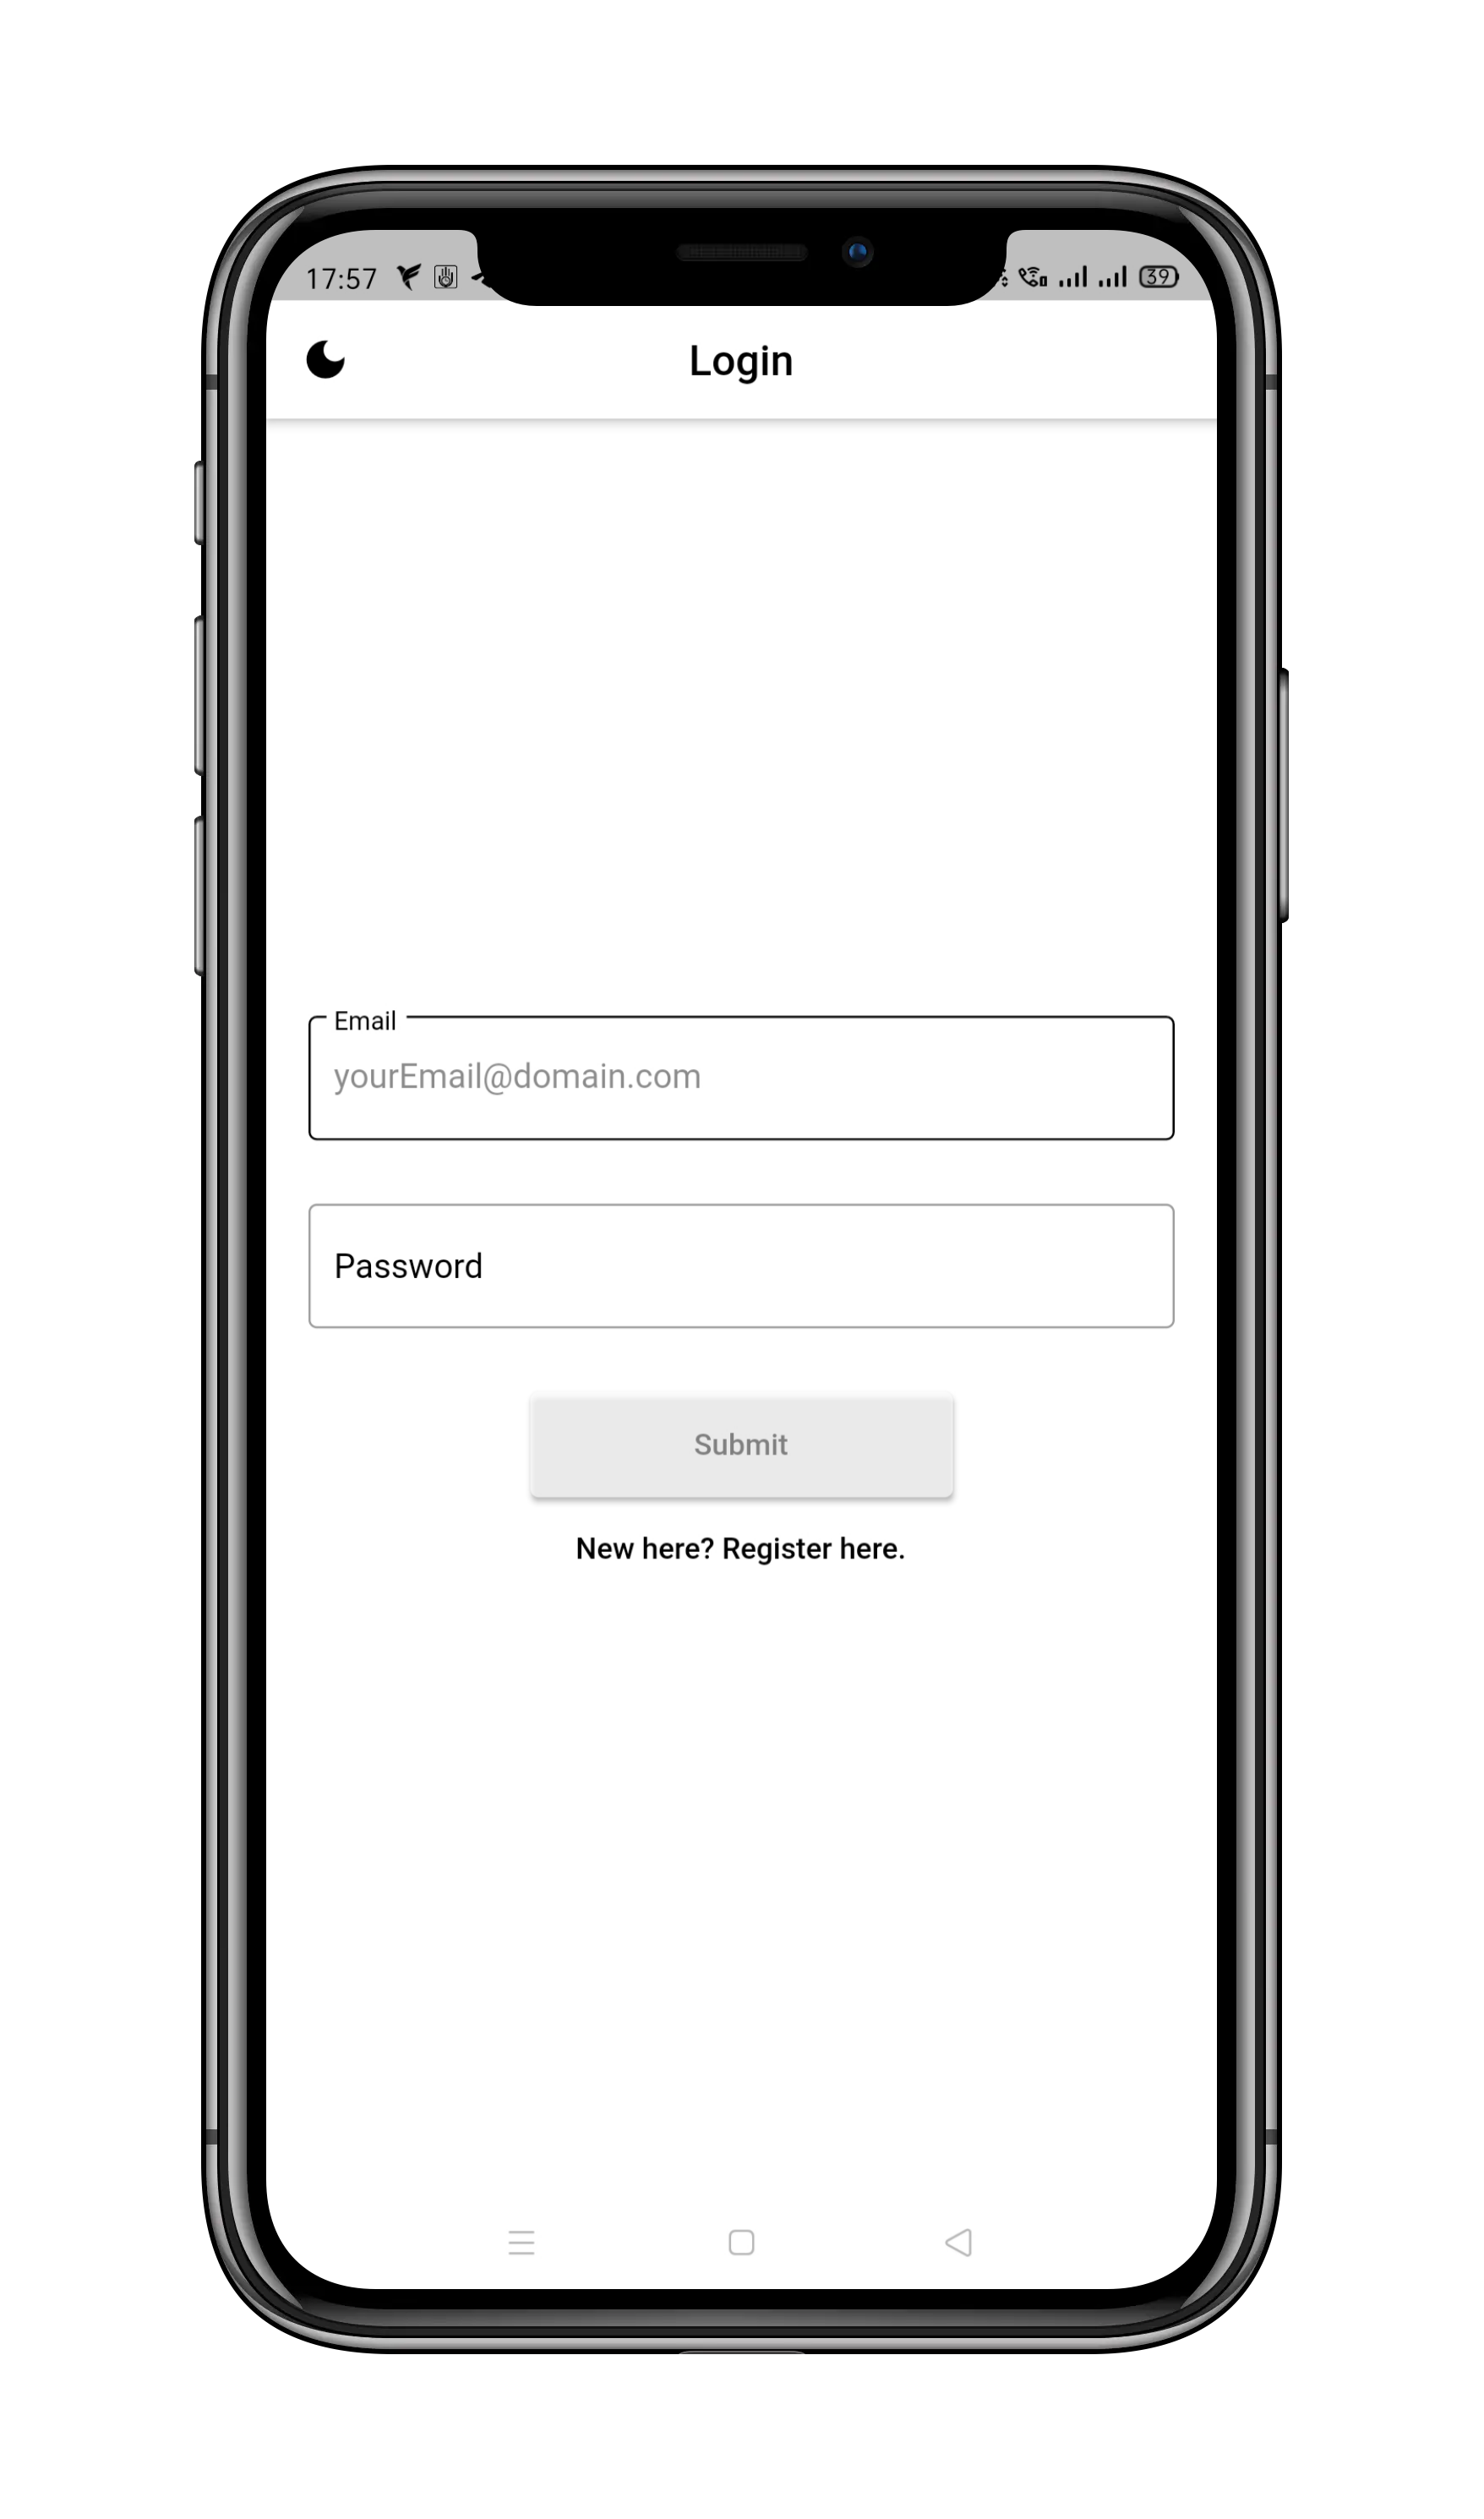
\includegraphics[height=90mm]{Images & Logos/theme/CH_08_Light_1.png}
  \caption{Login Page}
\end{minipage}%
\begin{minipage}{.5\textwidth}
  \centering
   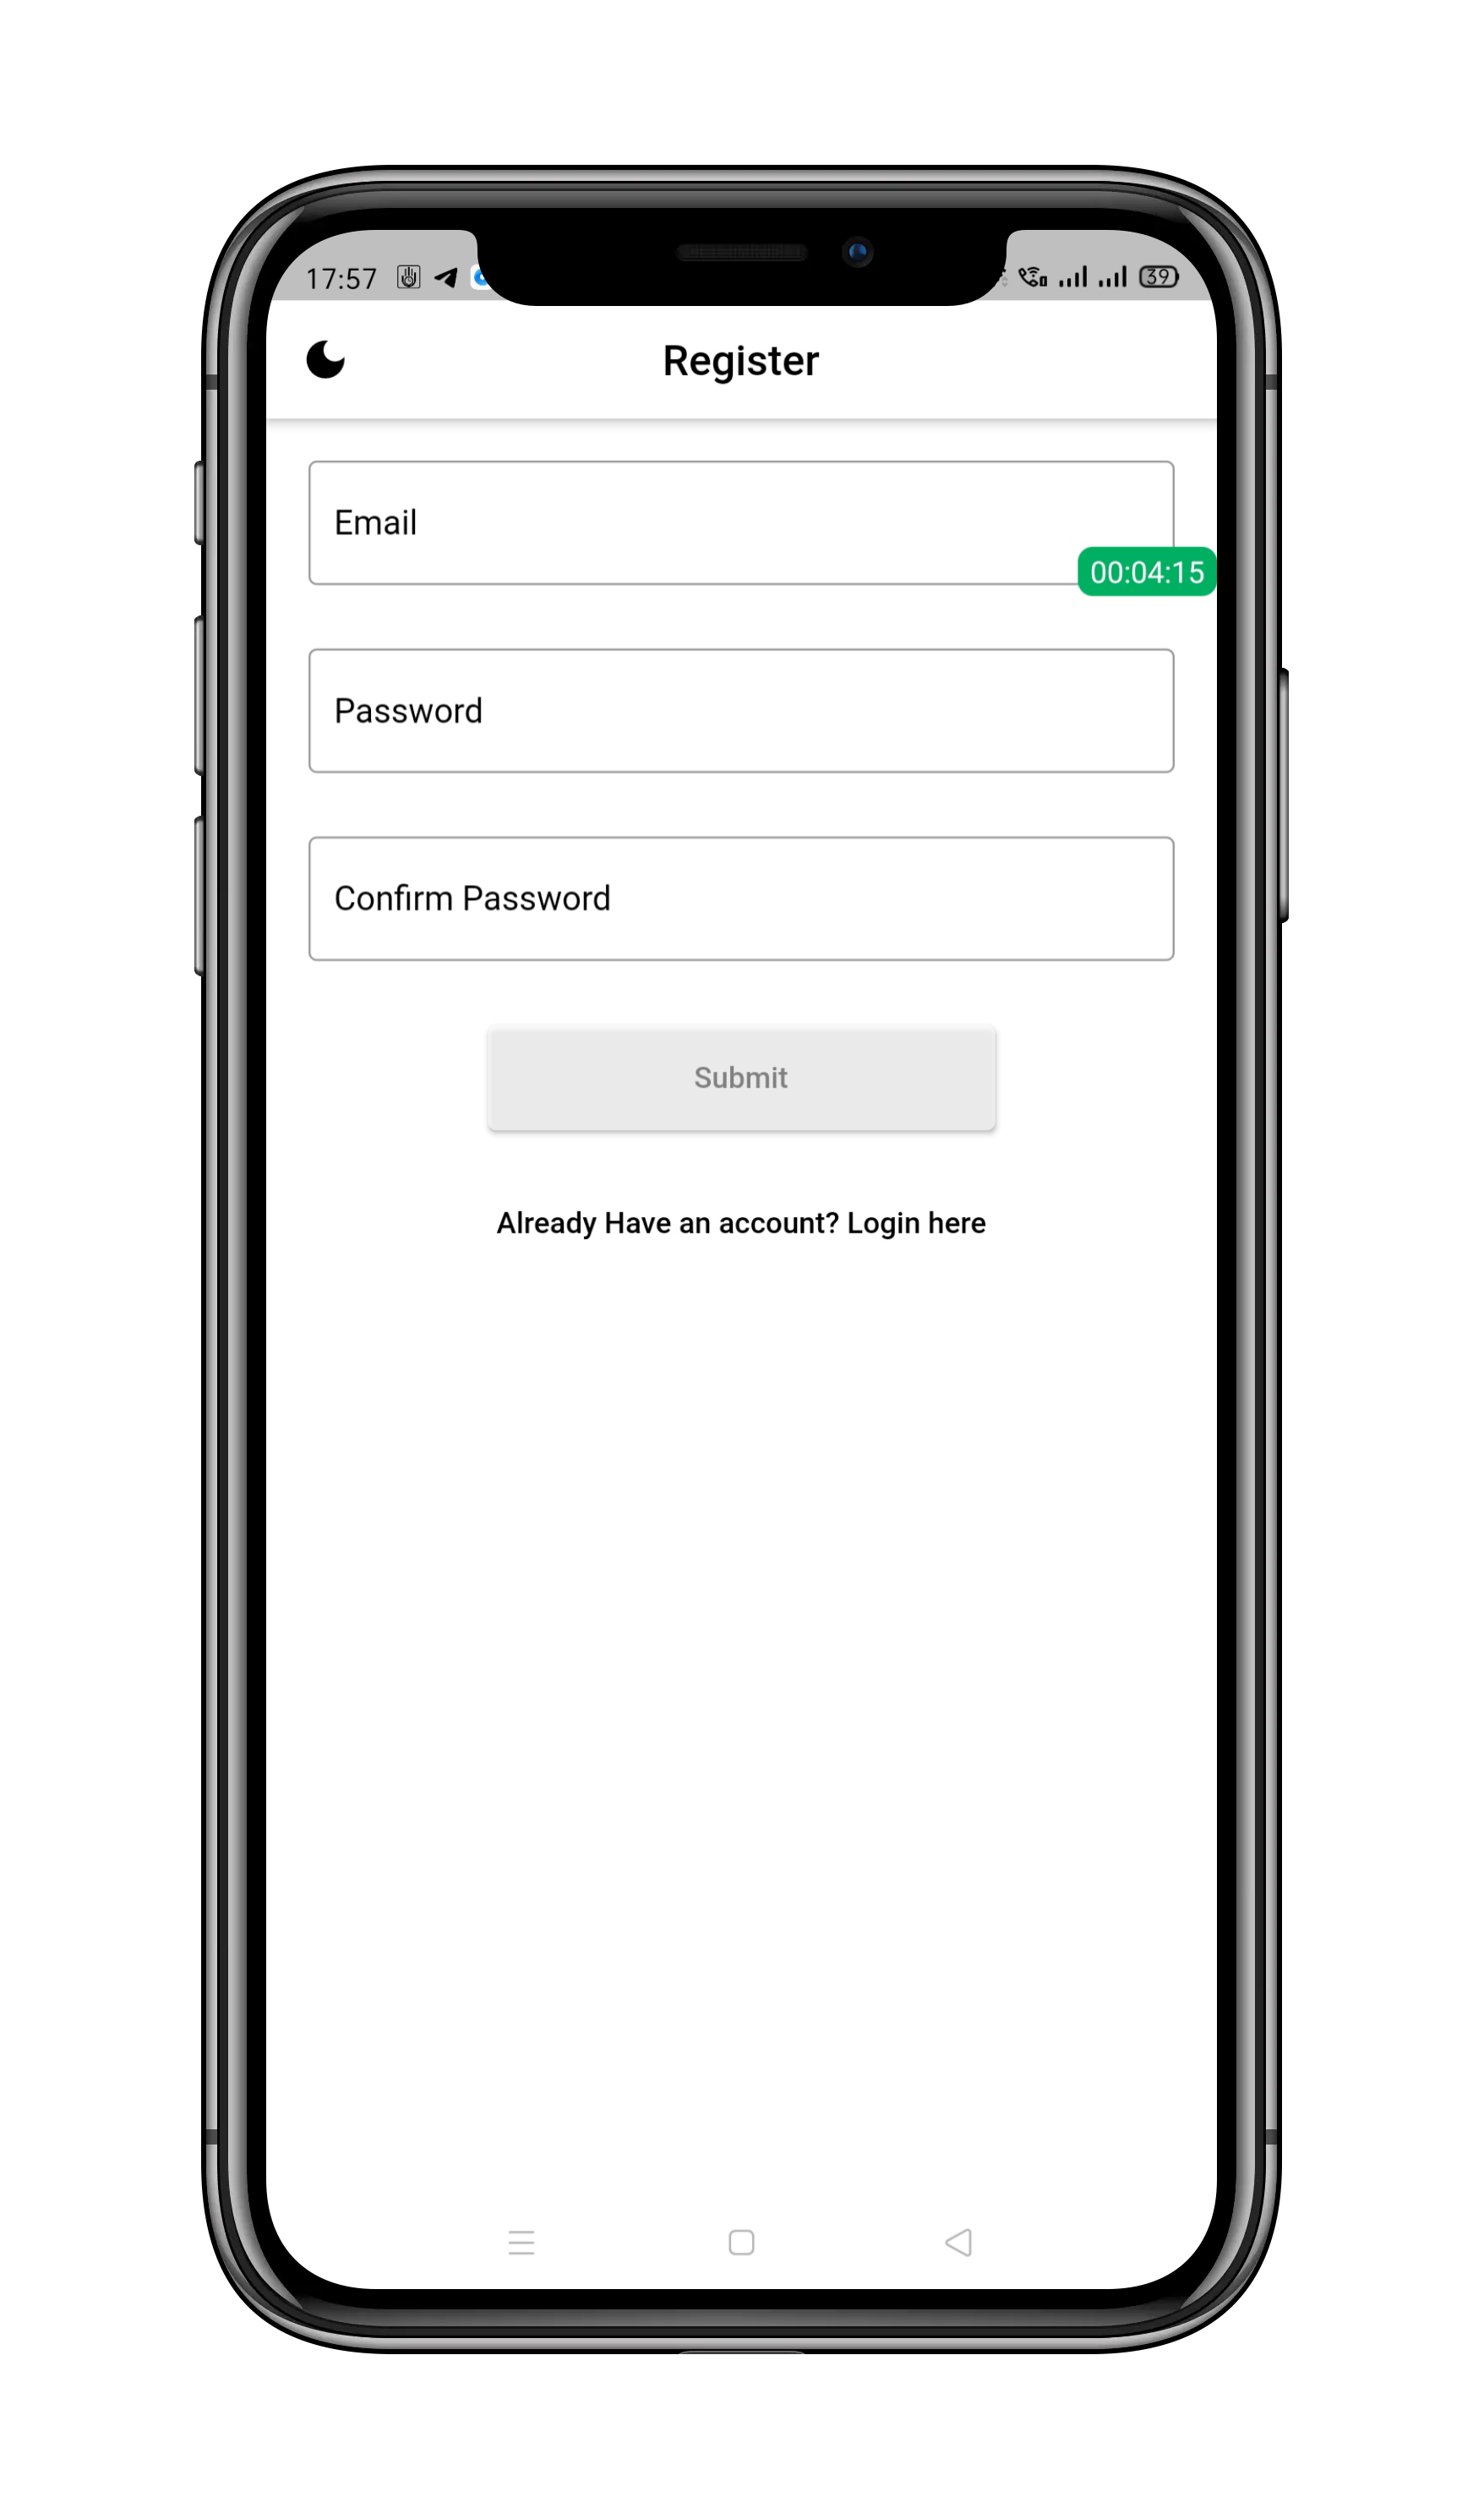
\includegraphics[height=90mm]{Images & Logos/theme/CH_08_Light_2.png}\\
  \caption{Registration page}
\end{minipage}

\centering
\begin{minipage}{.5\textwidth}
  \centering
   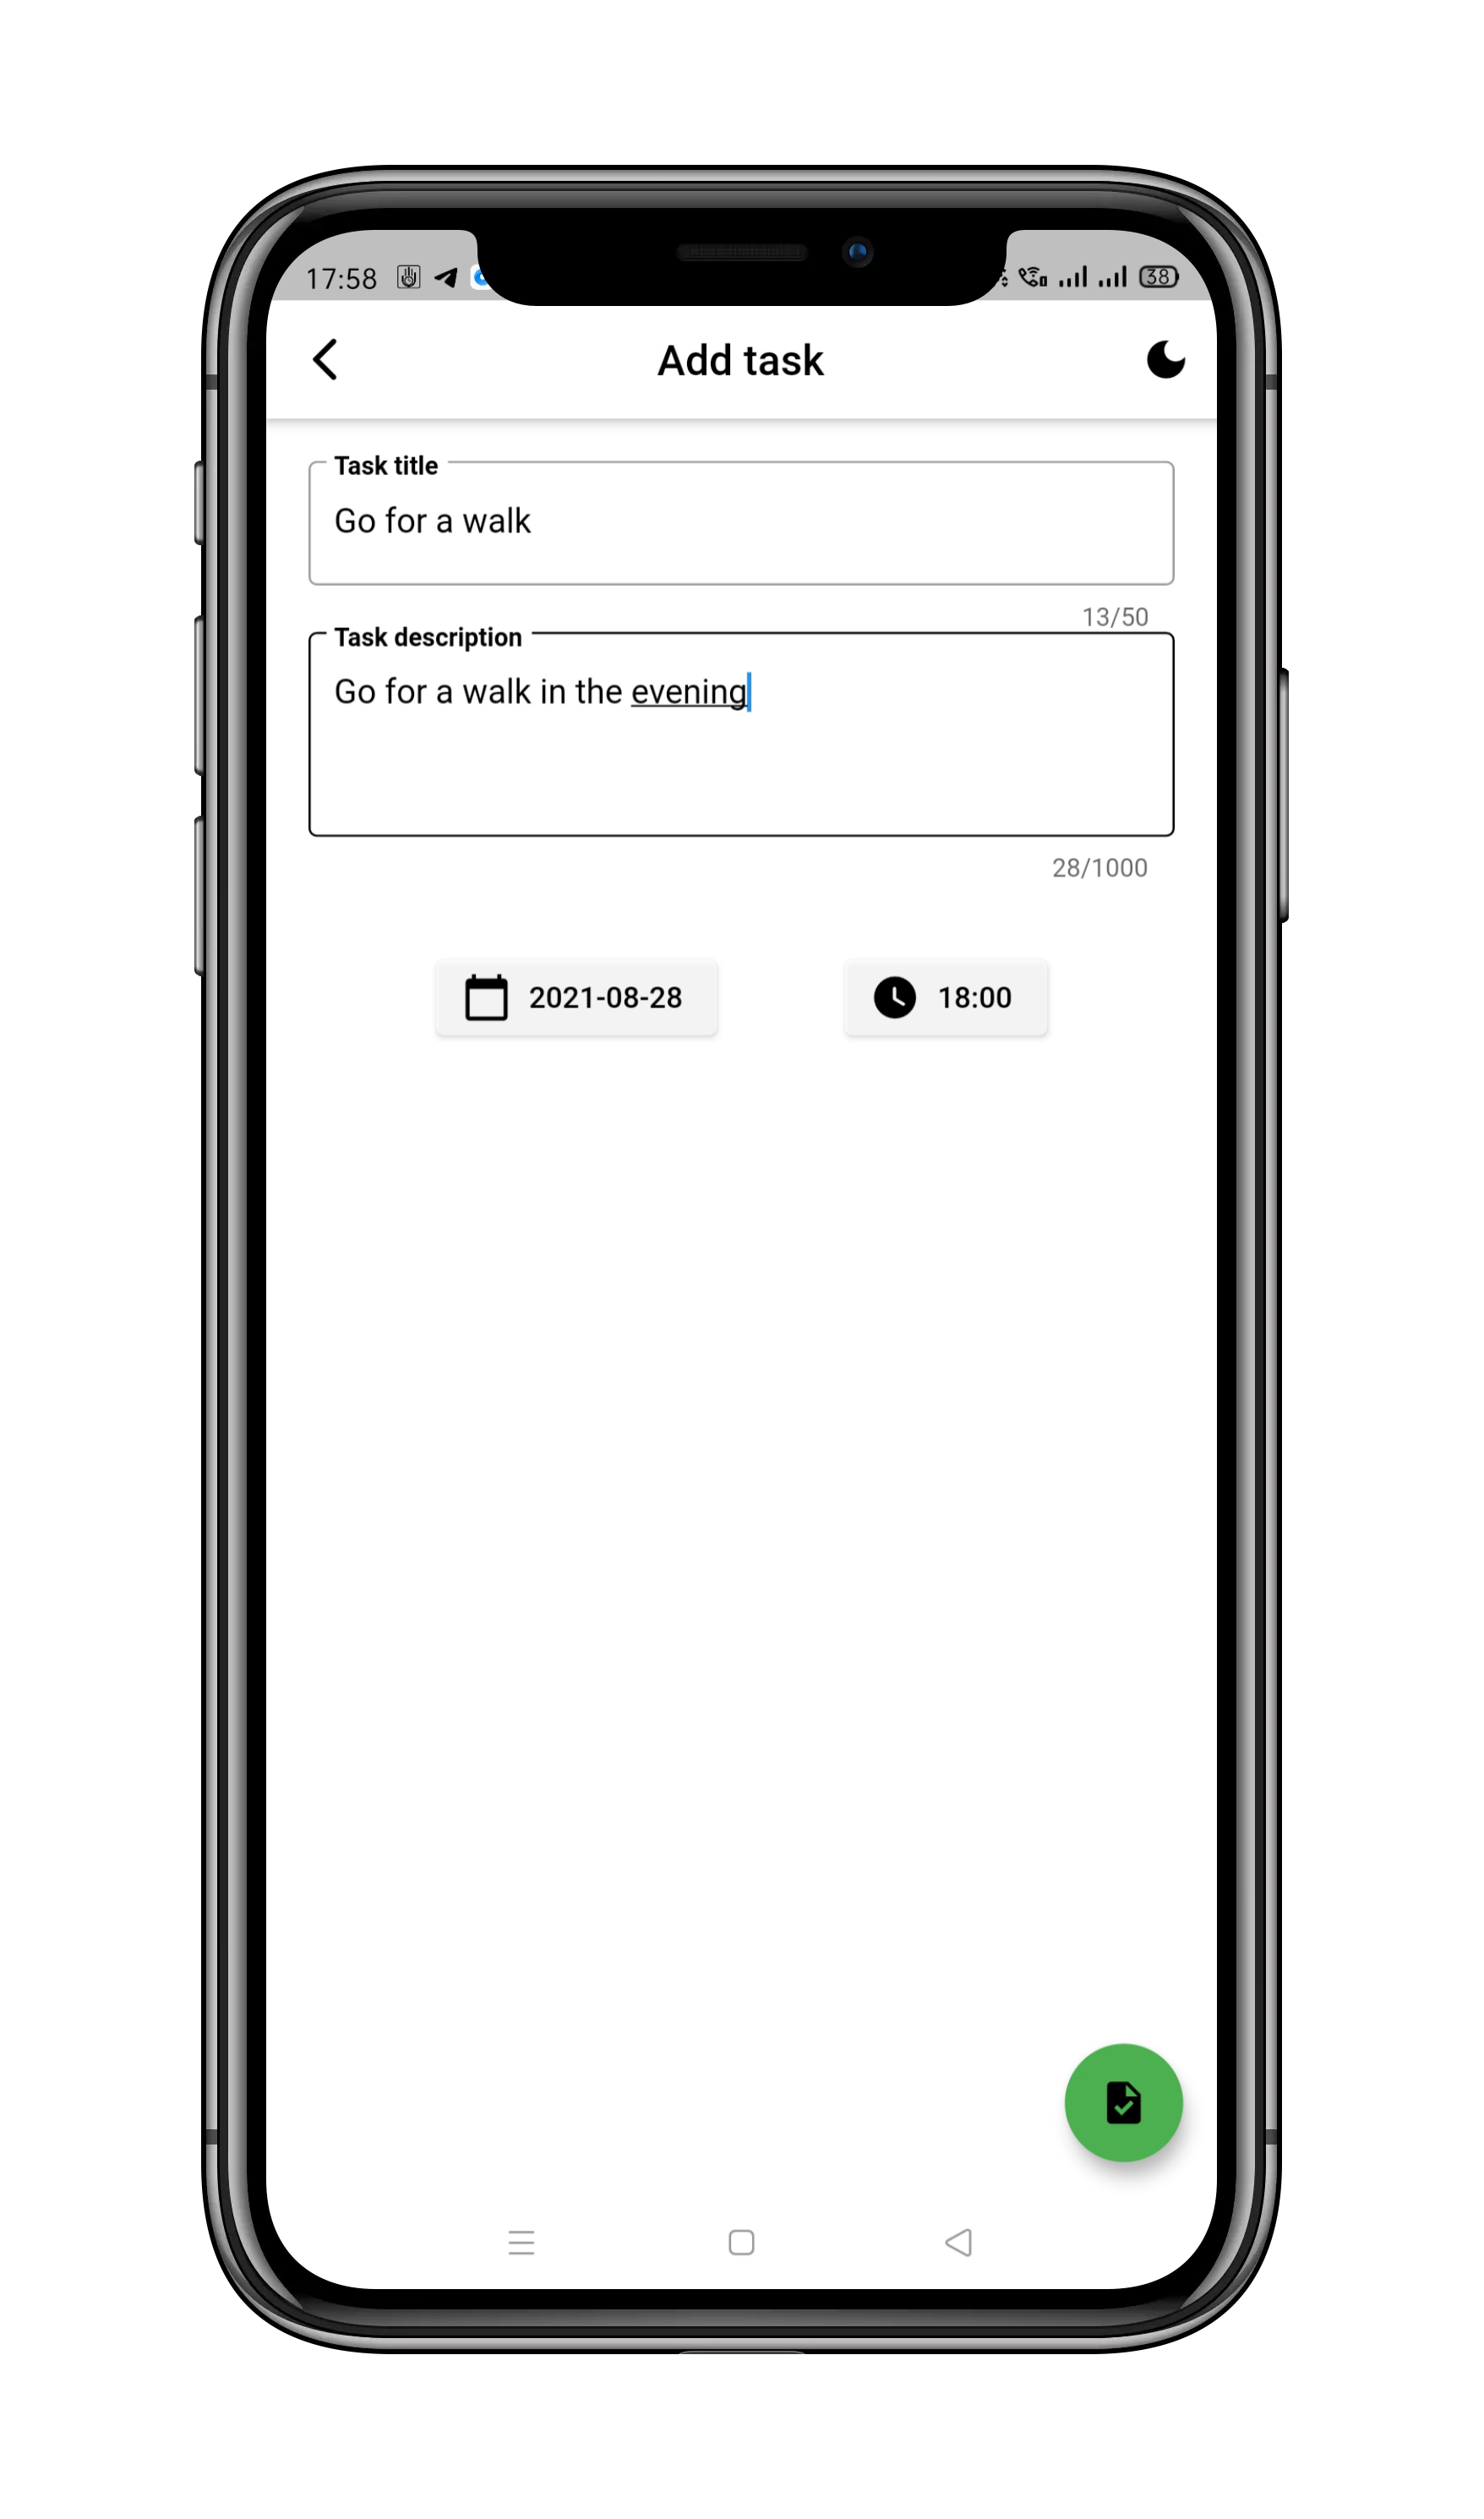
\includegraphics[height=90mm]{Images & Logos/theme/CH_08_Light_3.png}
  \caption{Add Task Page}
\end{minipage}%
\begin{minipage}{.5\textwidth}
  \centering
   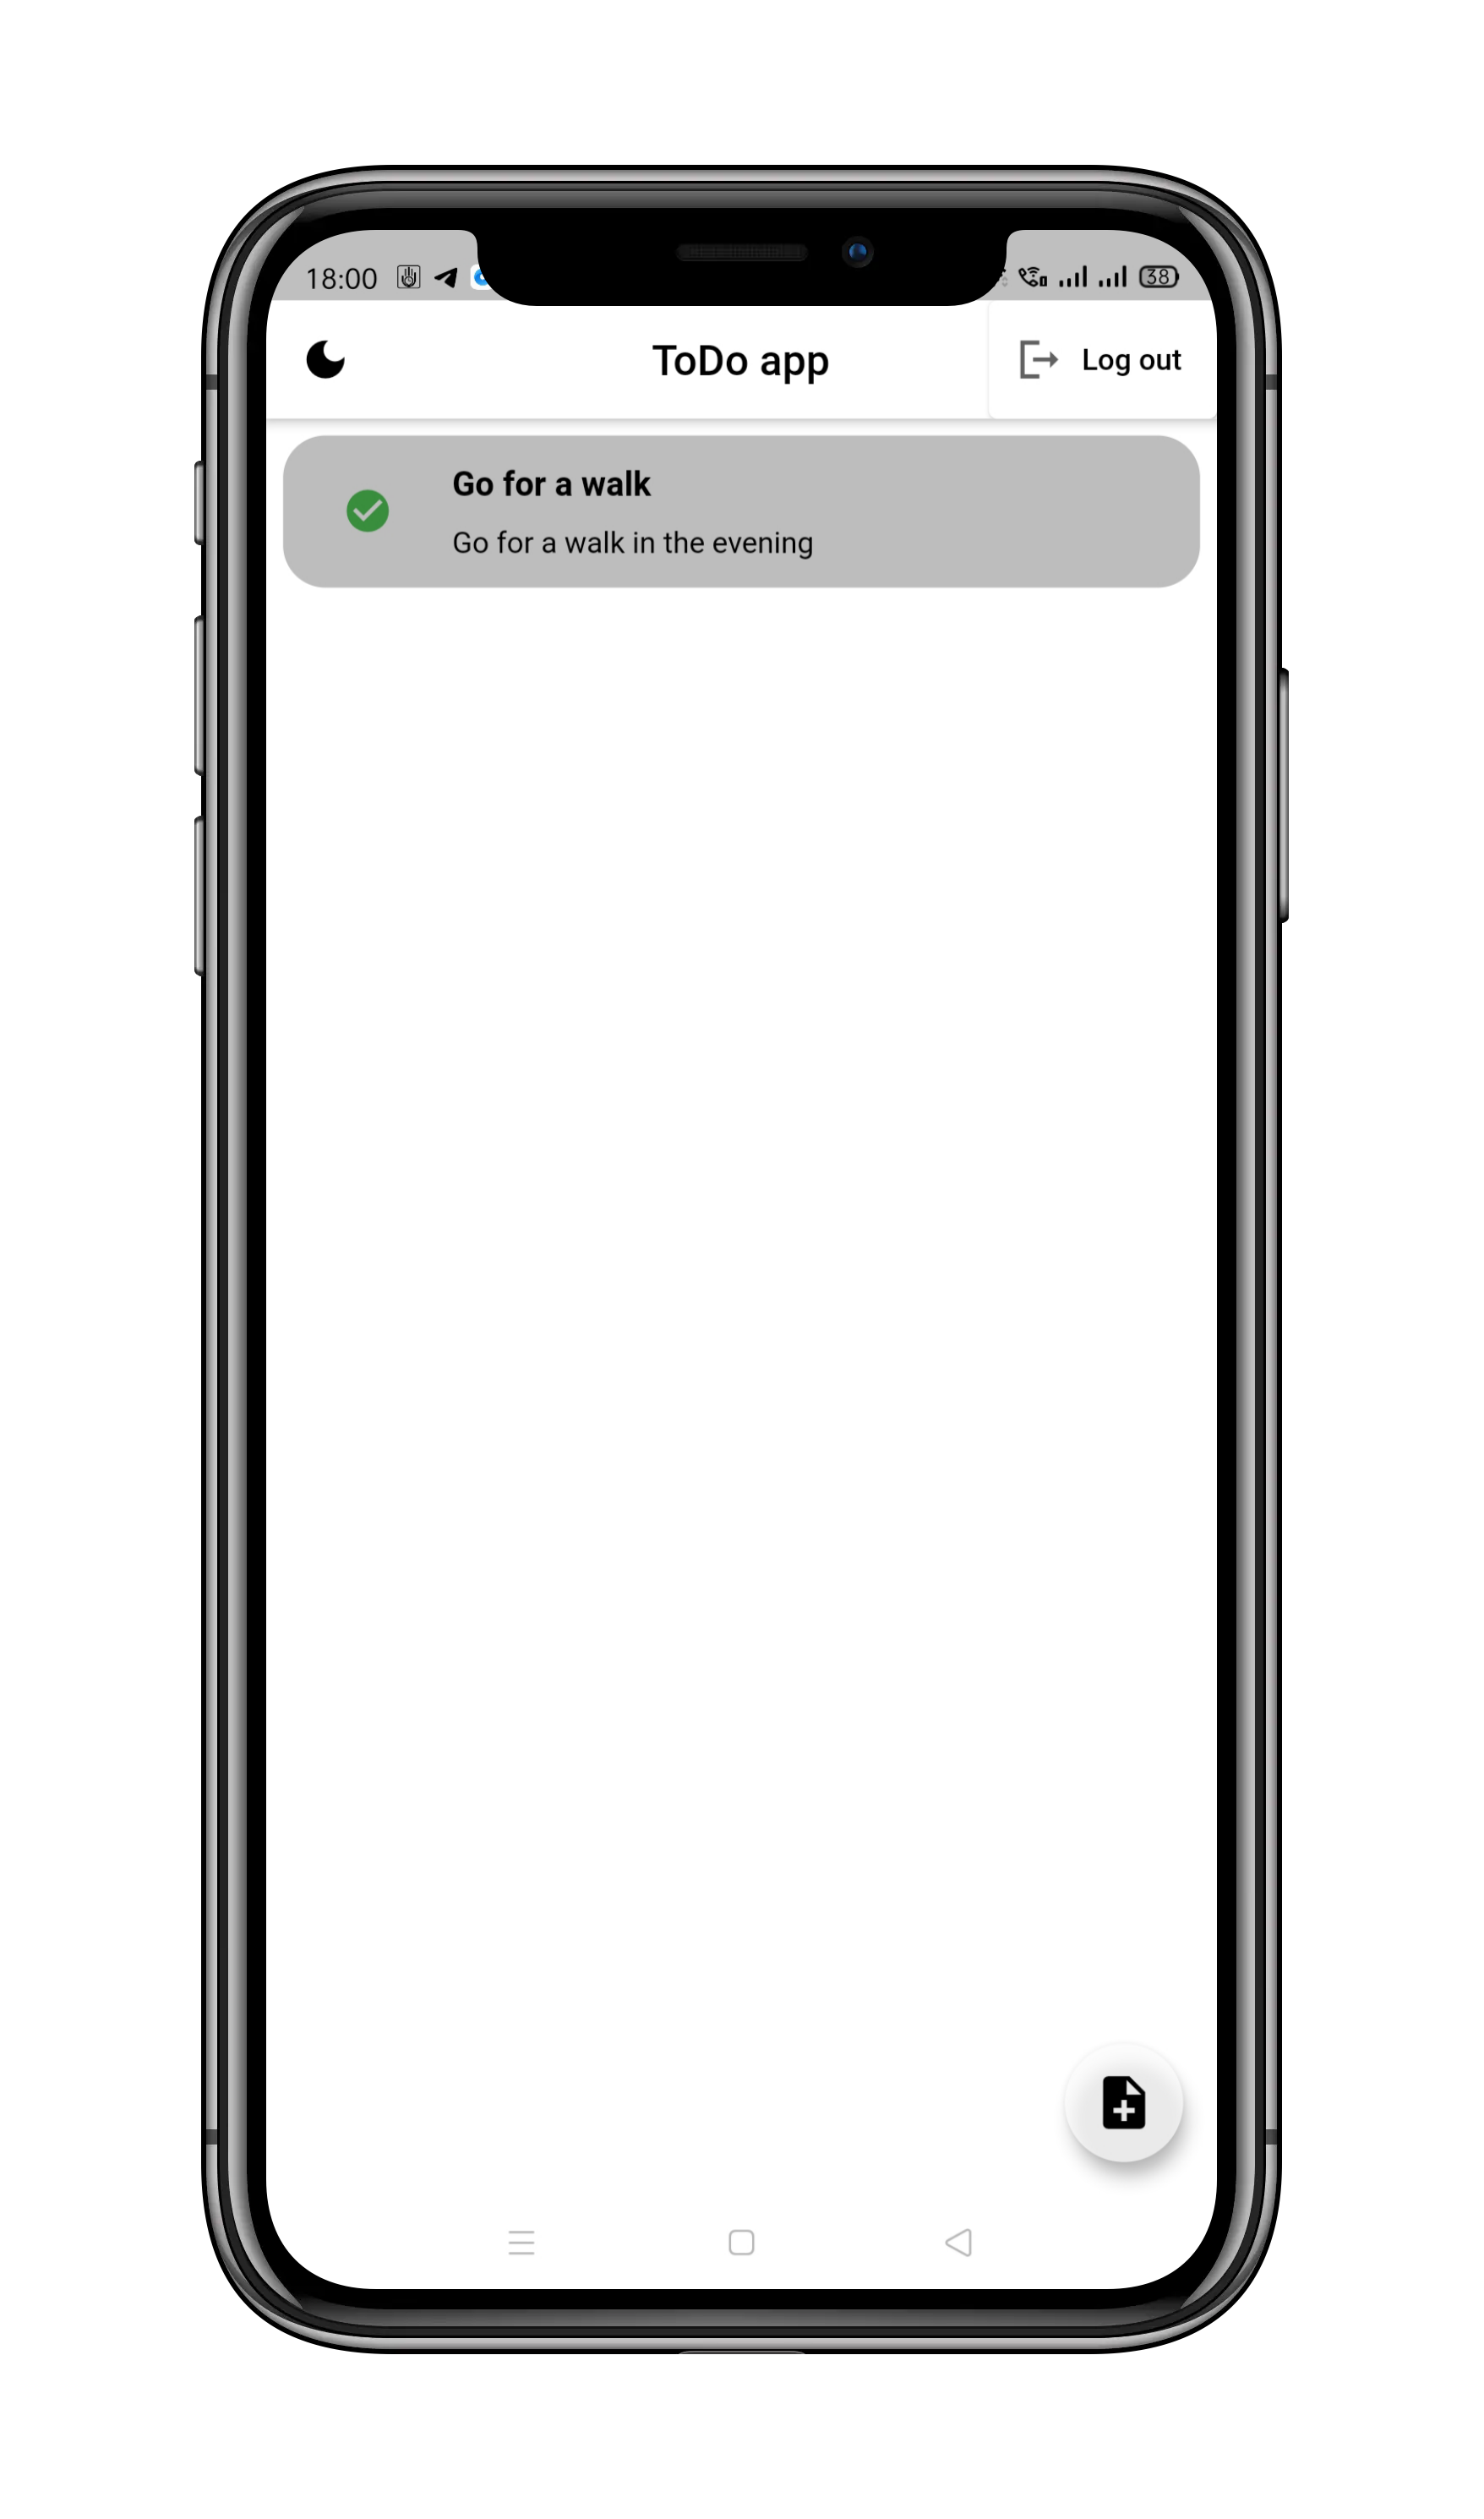
\includegraphics[height=90mm]{Images & Logos/theme/CH_08_Light_4.png}
  \caption{Home page}
\end{minipage}
\newpage
\end{figure}

\begin{figure}[h]
  \begin{center}
   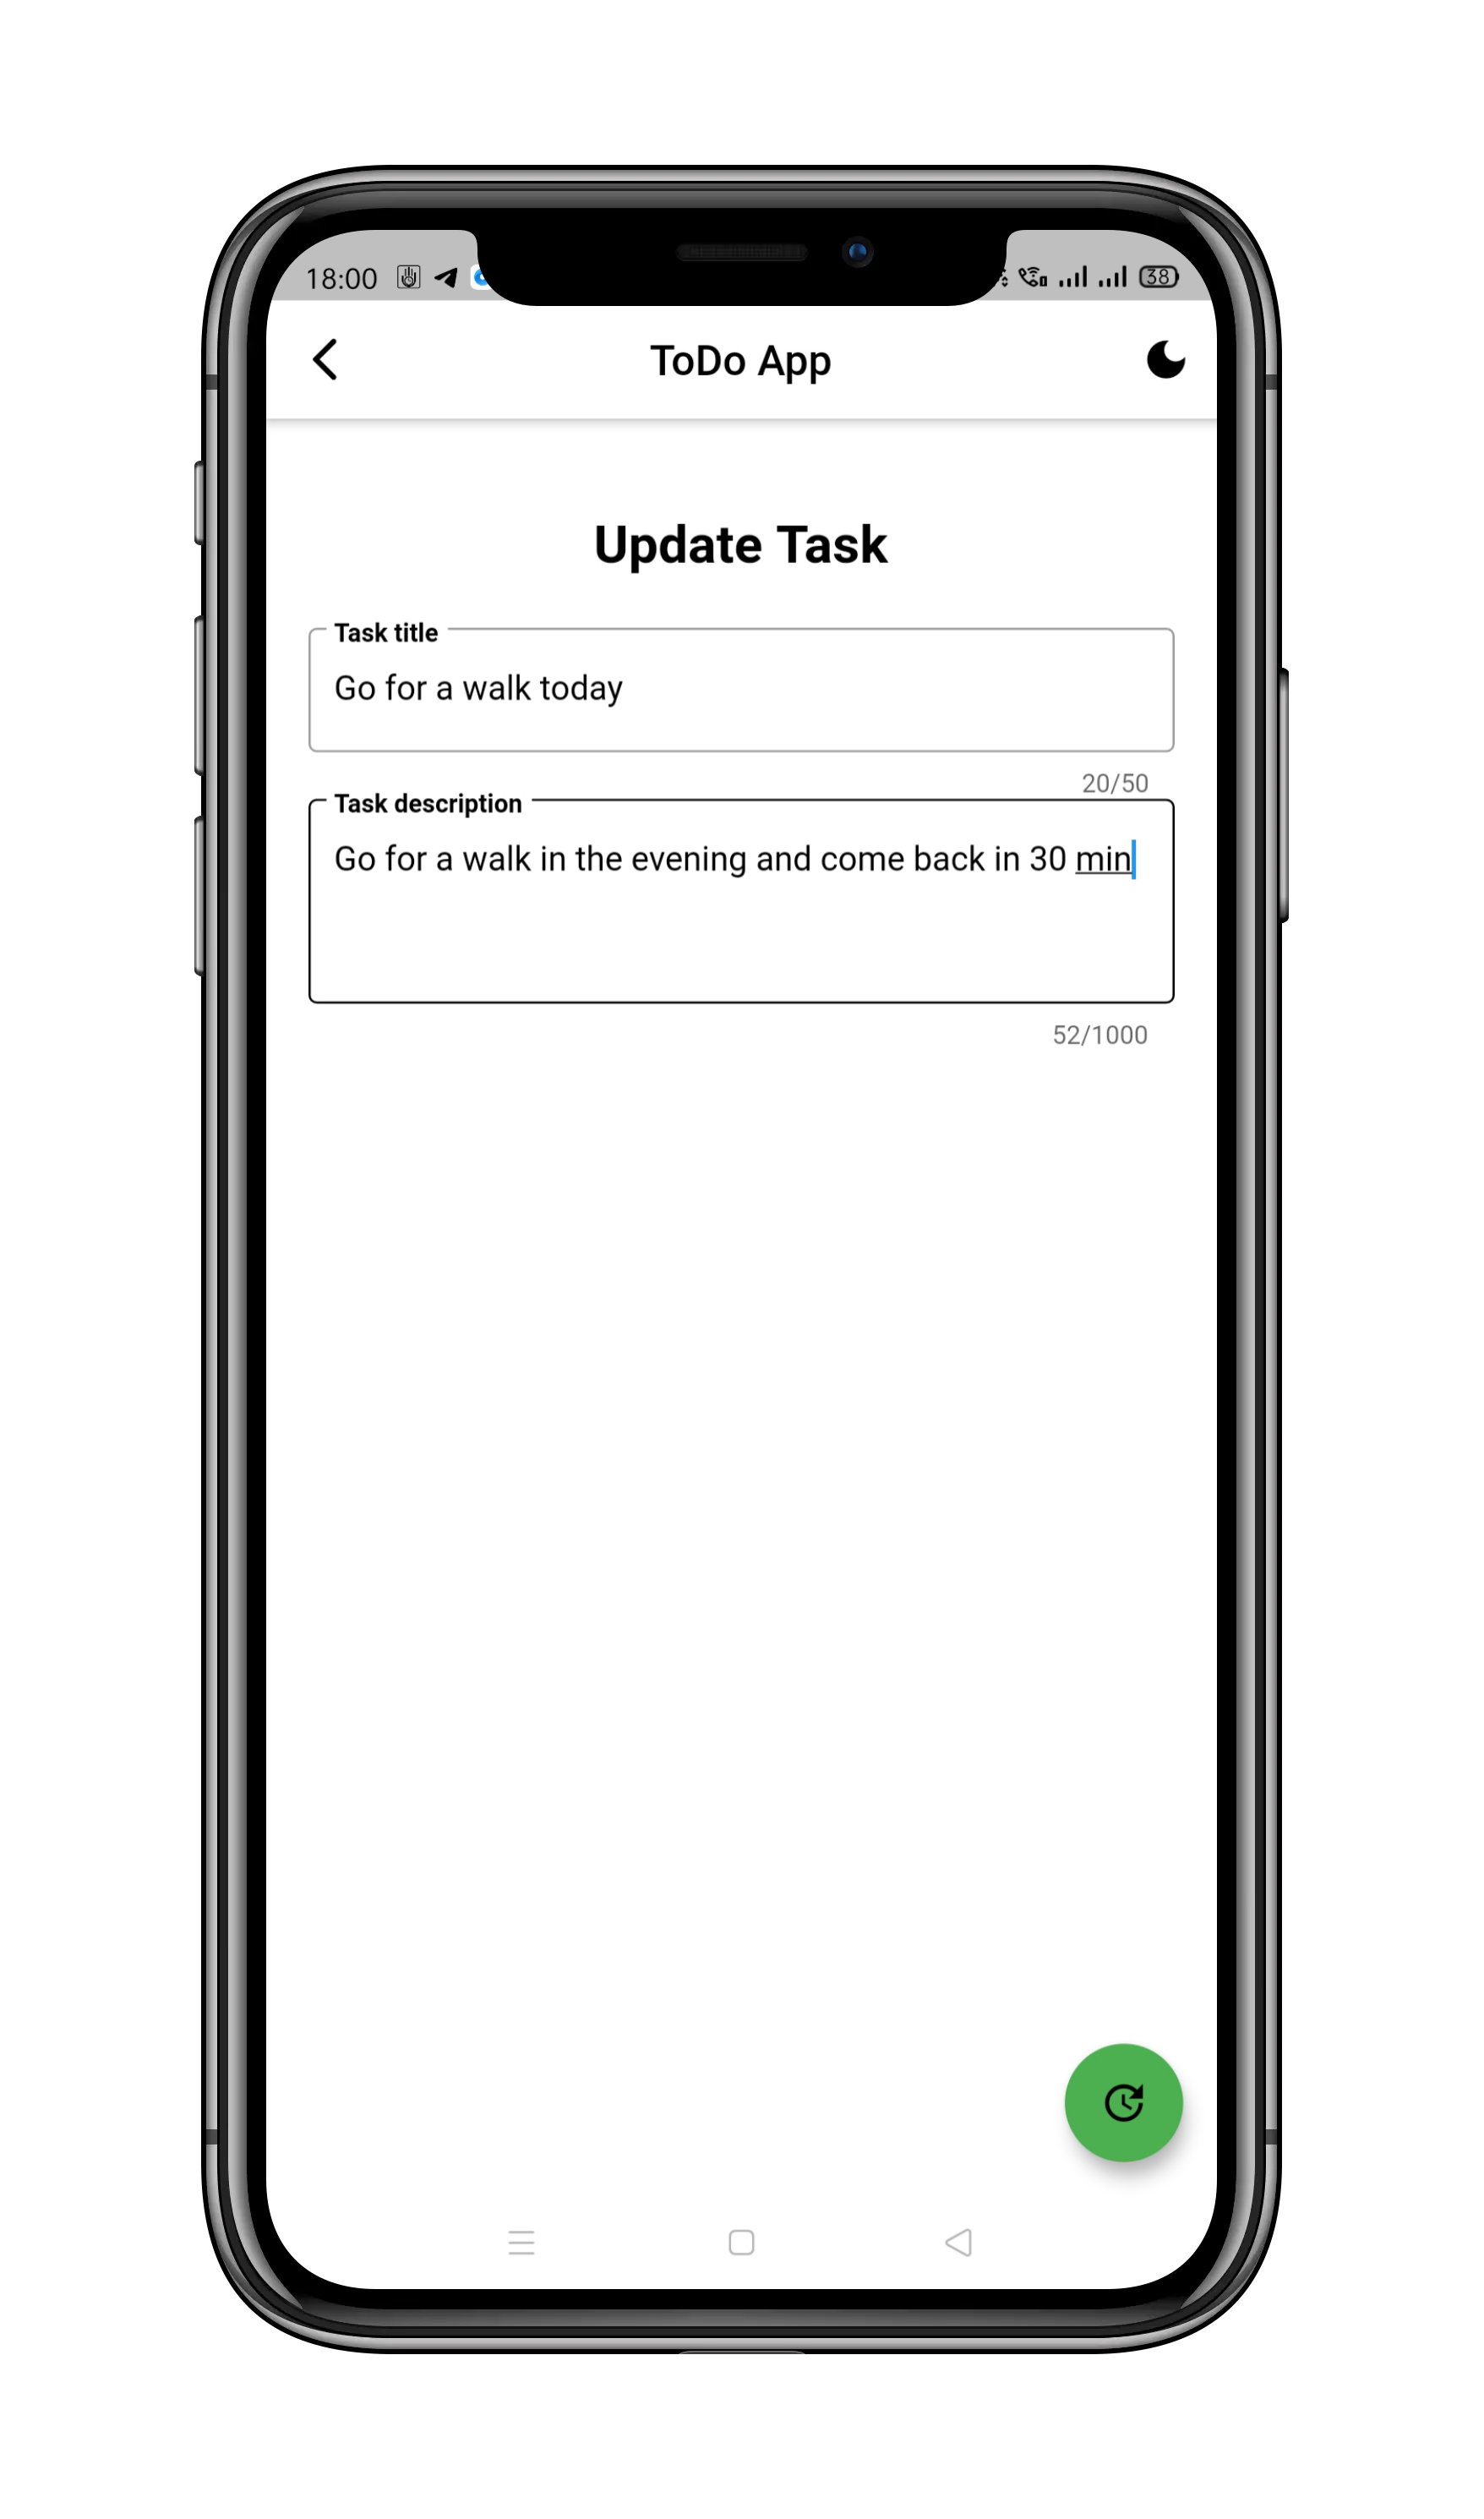
\includegraphics[height=90mm]{Images & Logos/theme/CH_08_Light_5.png}
%  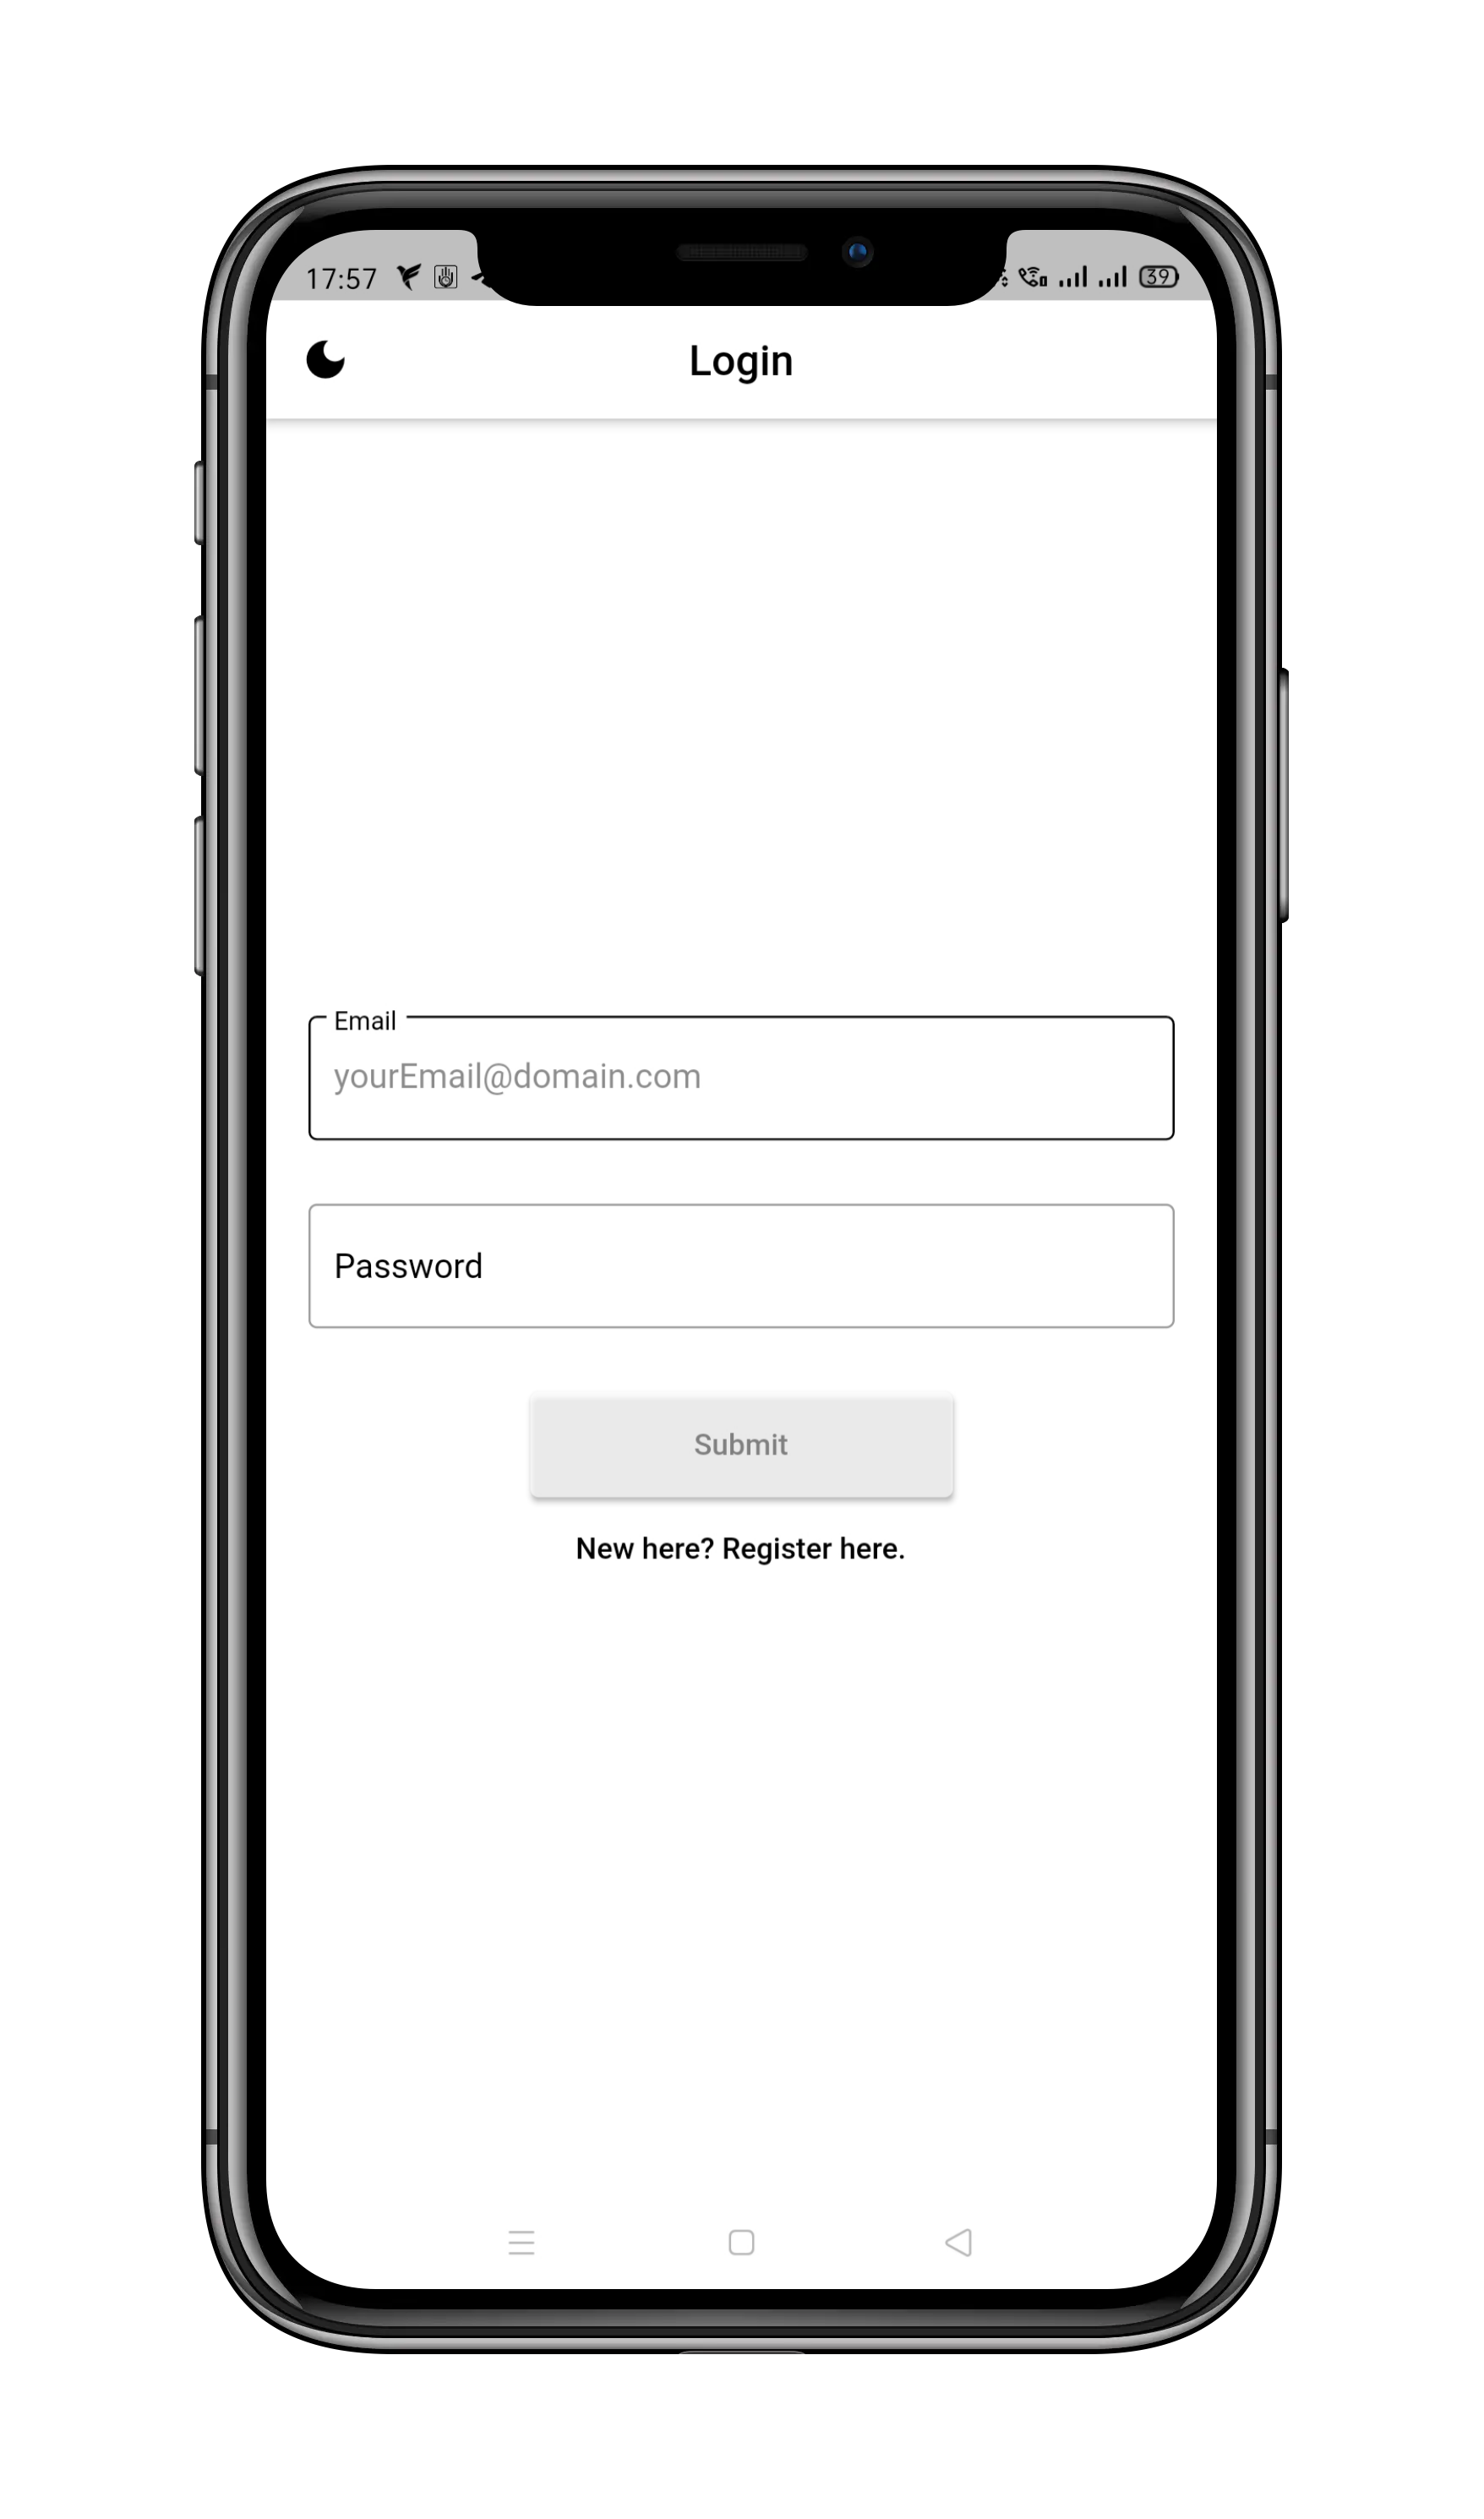
\includegraphics[height=70mm]{Images & Logos/theme/CH_08_Light_1.png}\\
  \end{center}
  \caption{Update Task Page}
\end{figure}  
\newpage
\hfill
\subsection{Dark Mode}
\begin{itemize}
\item An eye friendly shade of black as background of app (Hexcode: \#1A1A1A)
\item Black buttons with a silver-white outline
\item White icons
\item Green add task icon
\item Yellow color edit task icon
\end{itemize}

\begin{figure}
\centering
\begin{minipage}{.5\textwidth}
  \centering
   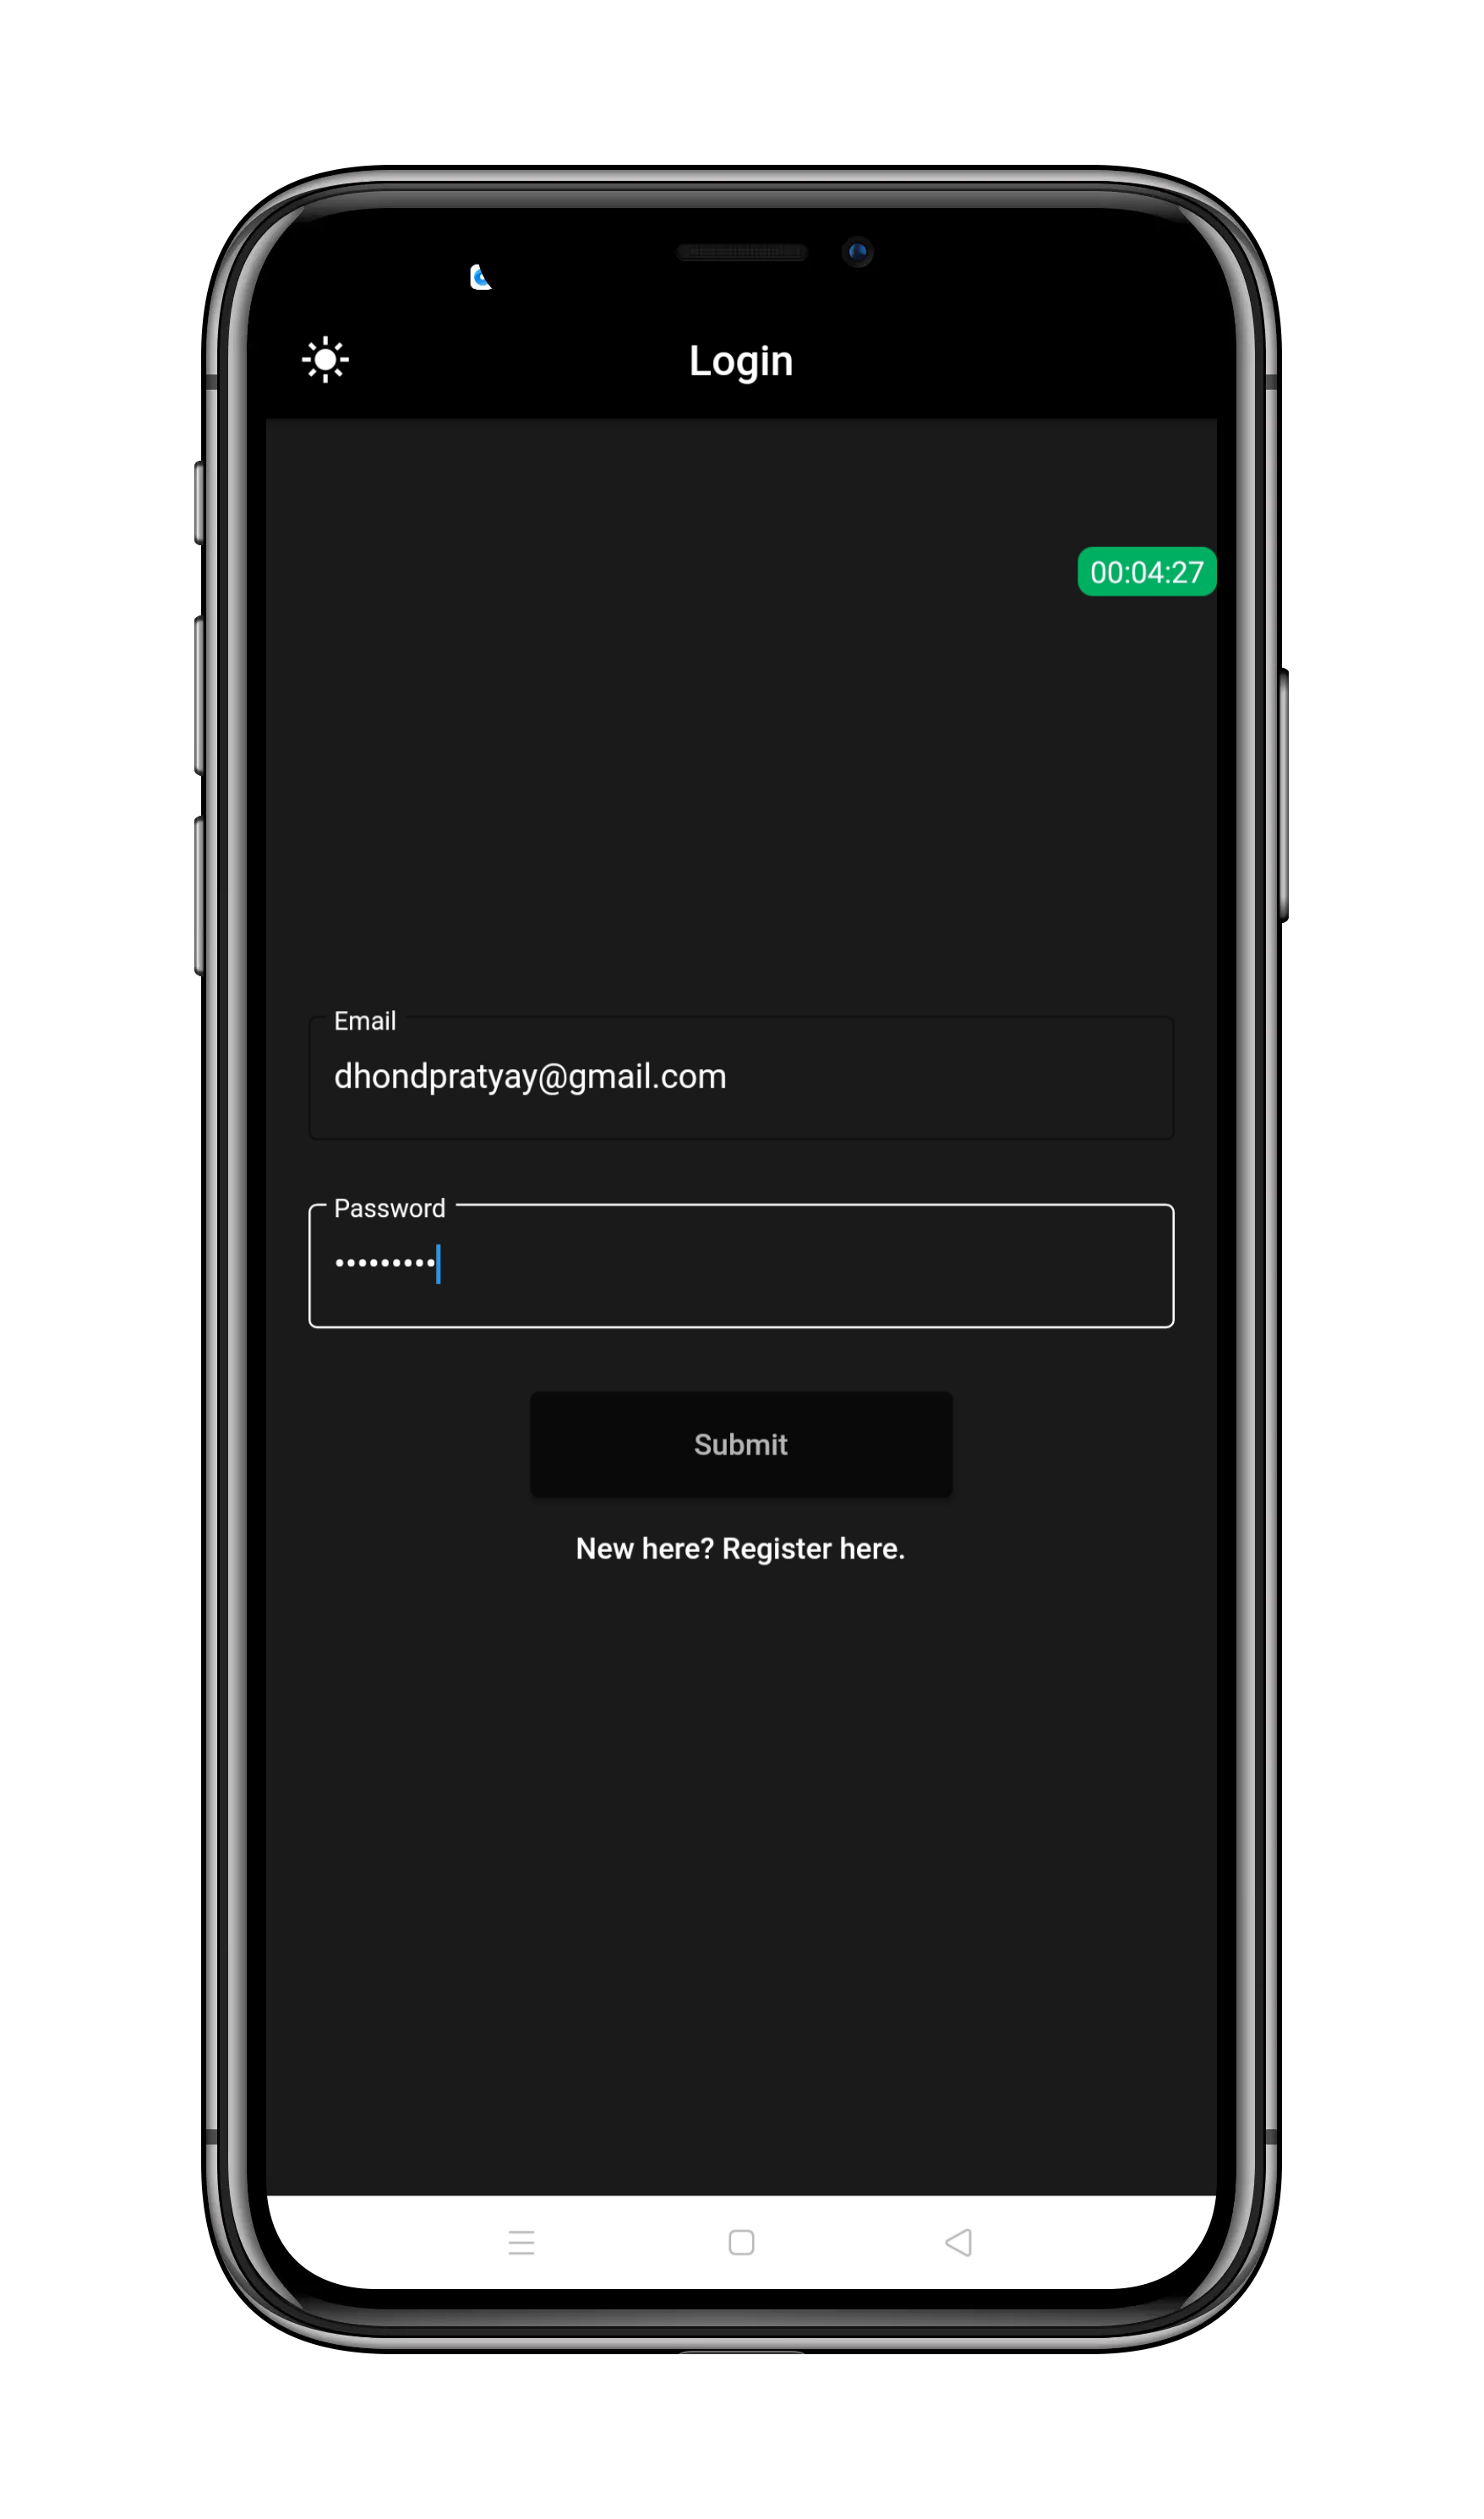
\includegraphics[height=90mm]{Images & Logos/theme/CH_08_Dark_1.png}
  \caption{Login Page}
\end{minipage}%
\begin{minipage}{.5\textwidth}
  \centering
   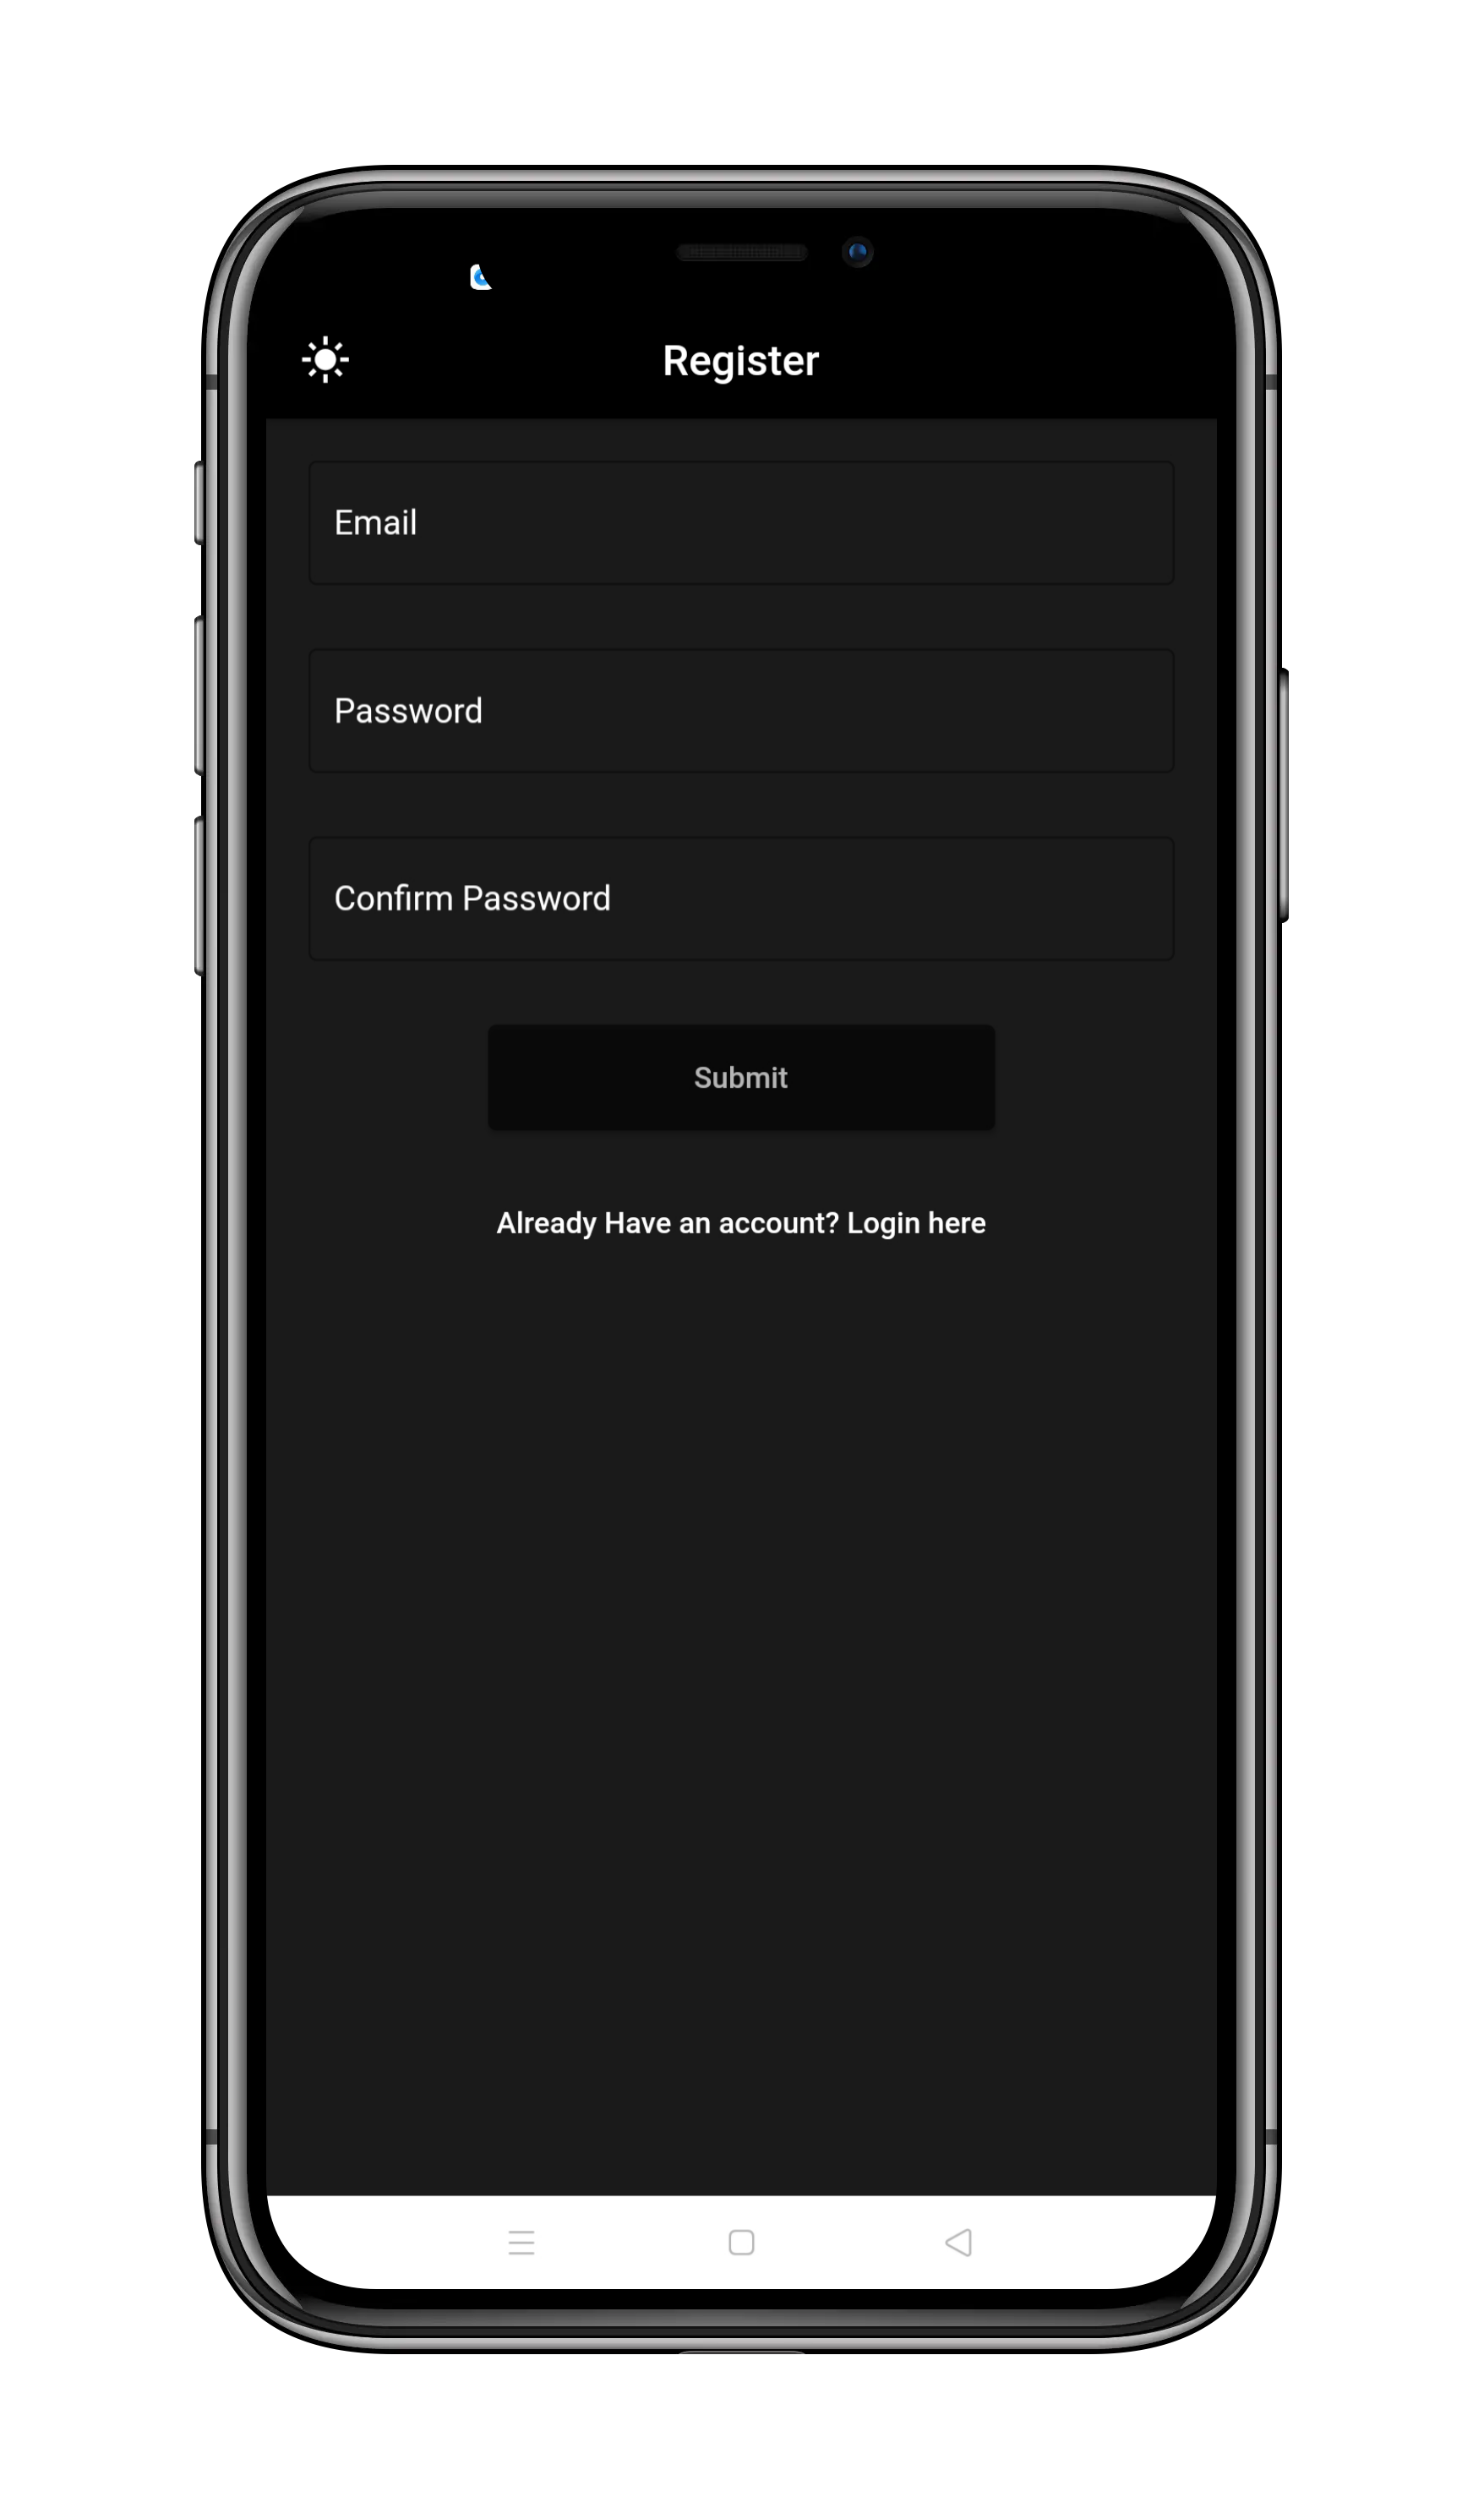
\includegraphics[height=90mm]{Images & Logos/theme/CH_08_Dark_2.png}\\
  \caption{Registration page}
\end{minipage}

\centering
\begin{minipage}{.5\textwidth}
  \centering
   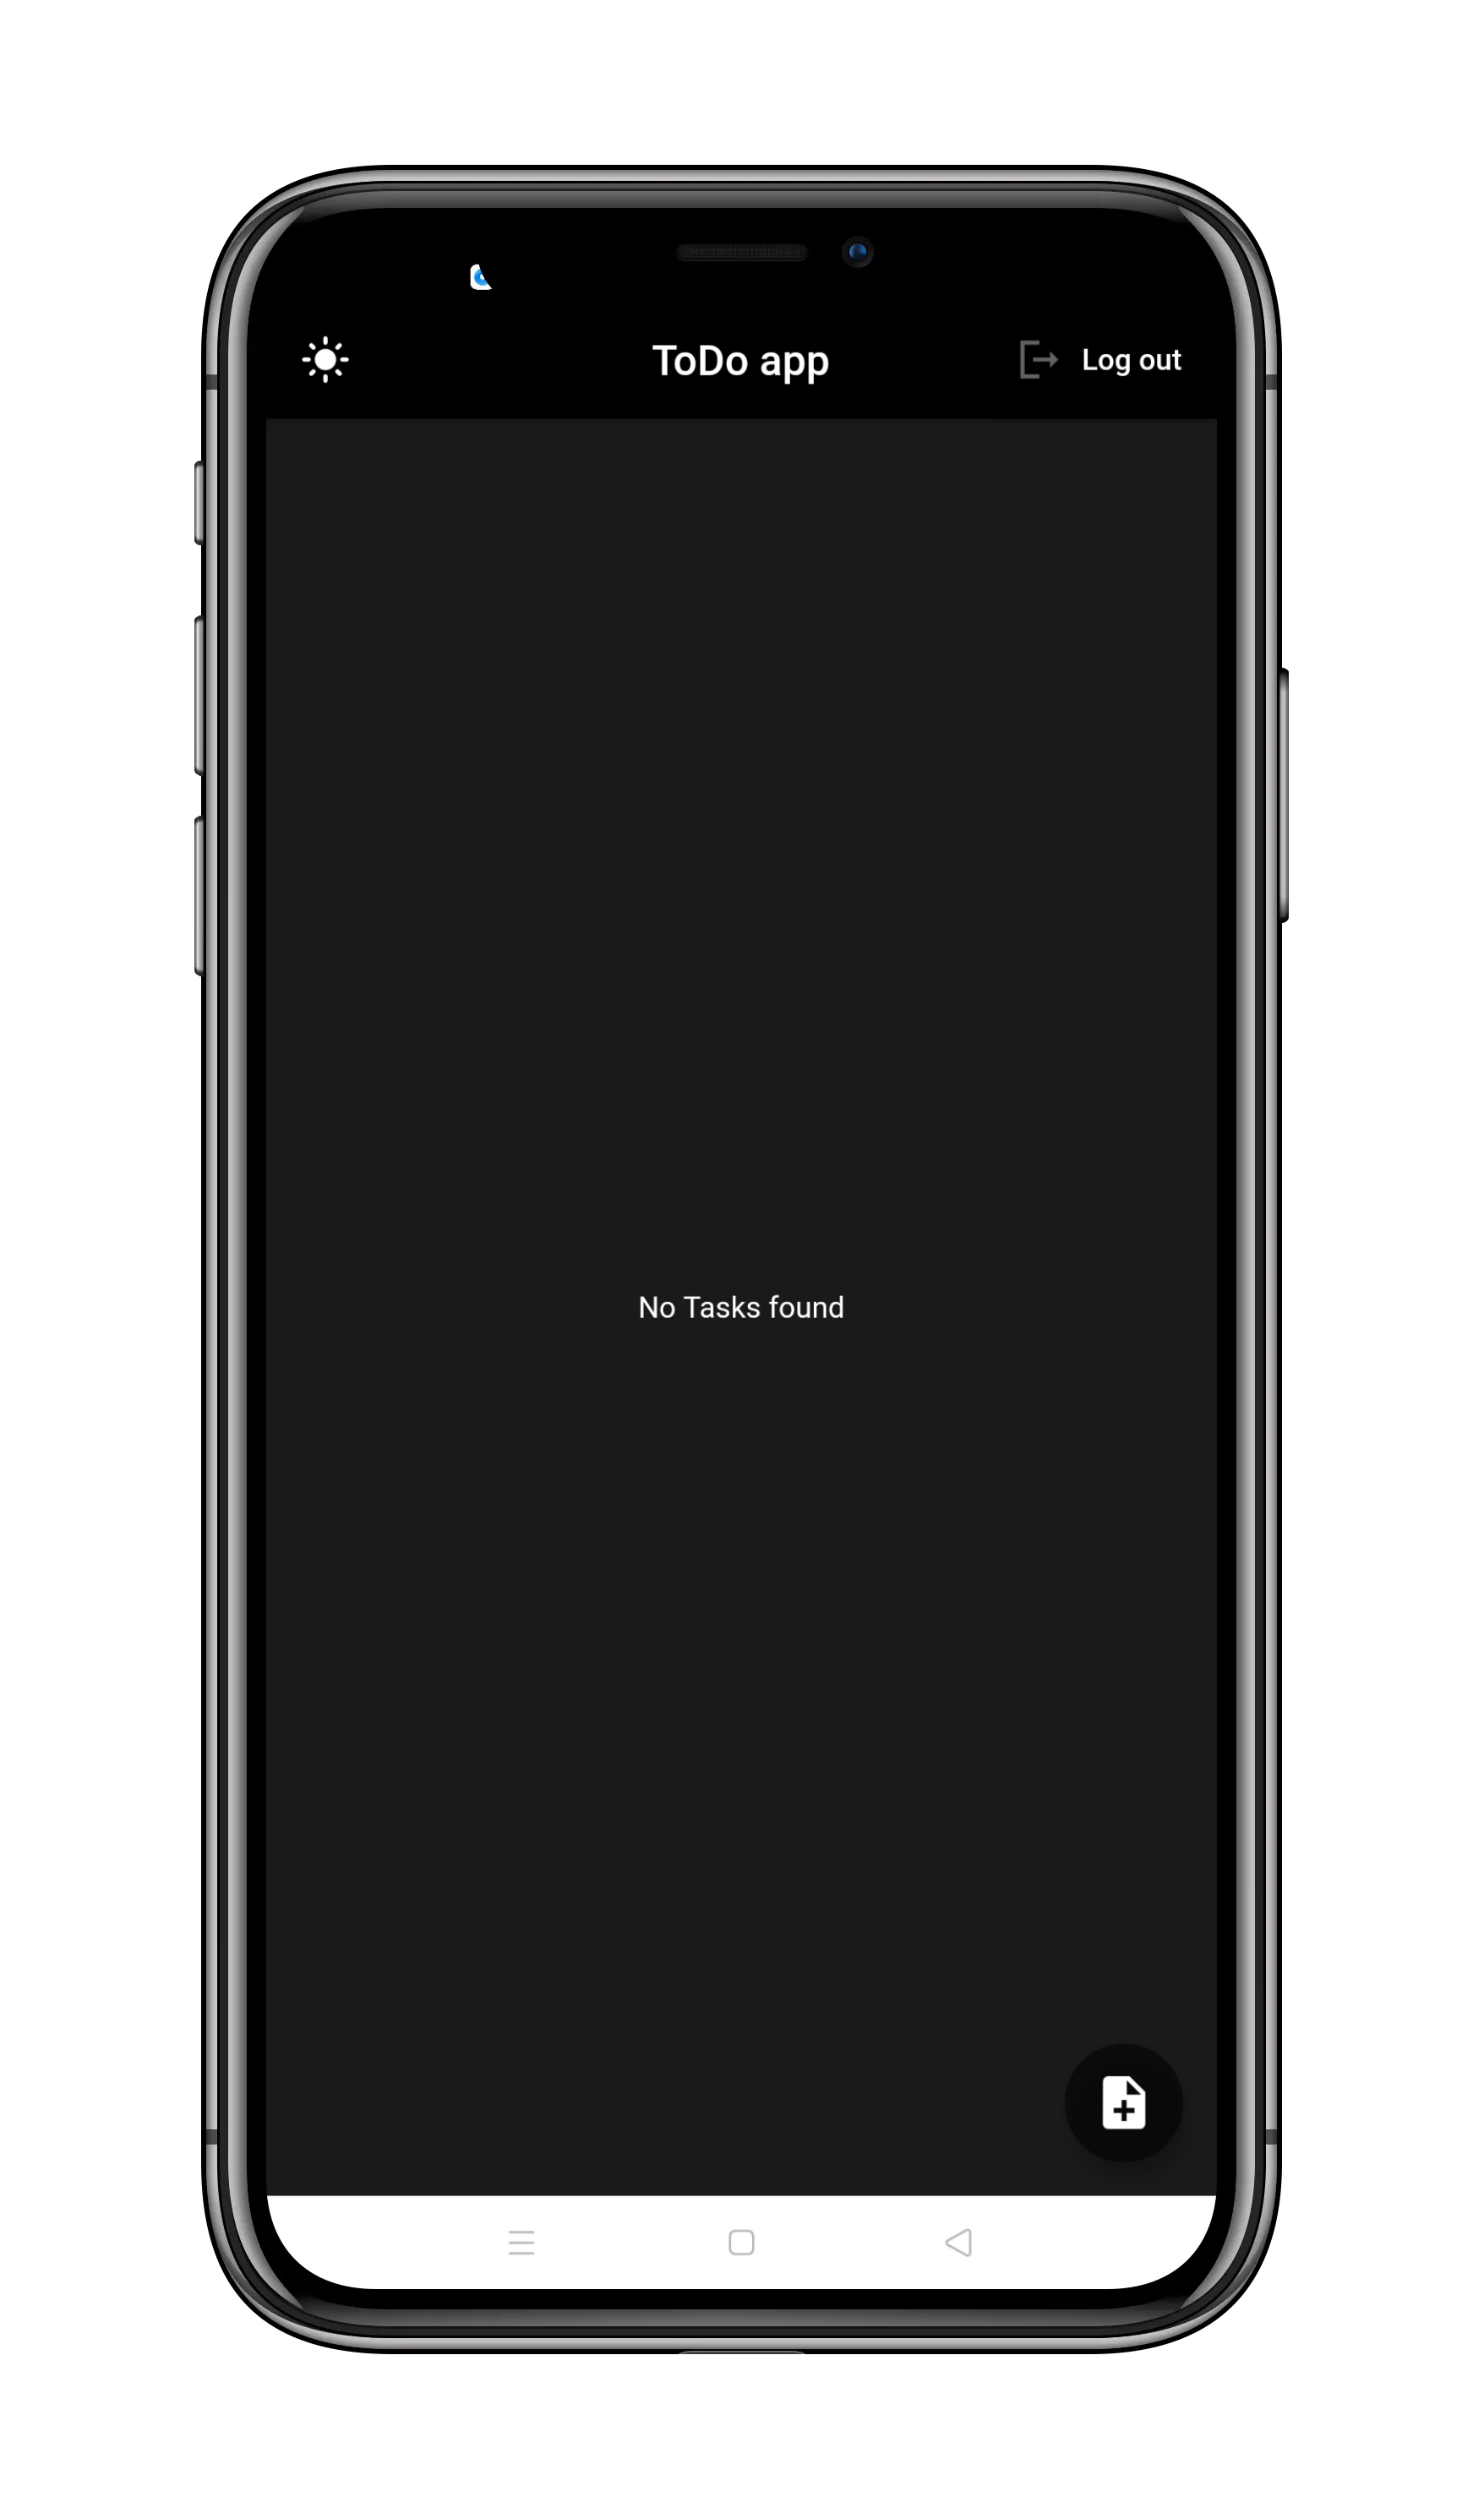
\includegraphics[height=90mm]{Images & Logos/theme/CH_08_Dark_3.png}
  \caption{Home Page}
\end{minipage}%
\begin{minipage}{.5\textwidth}
  \centering
   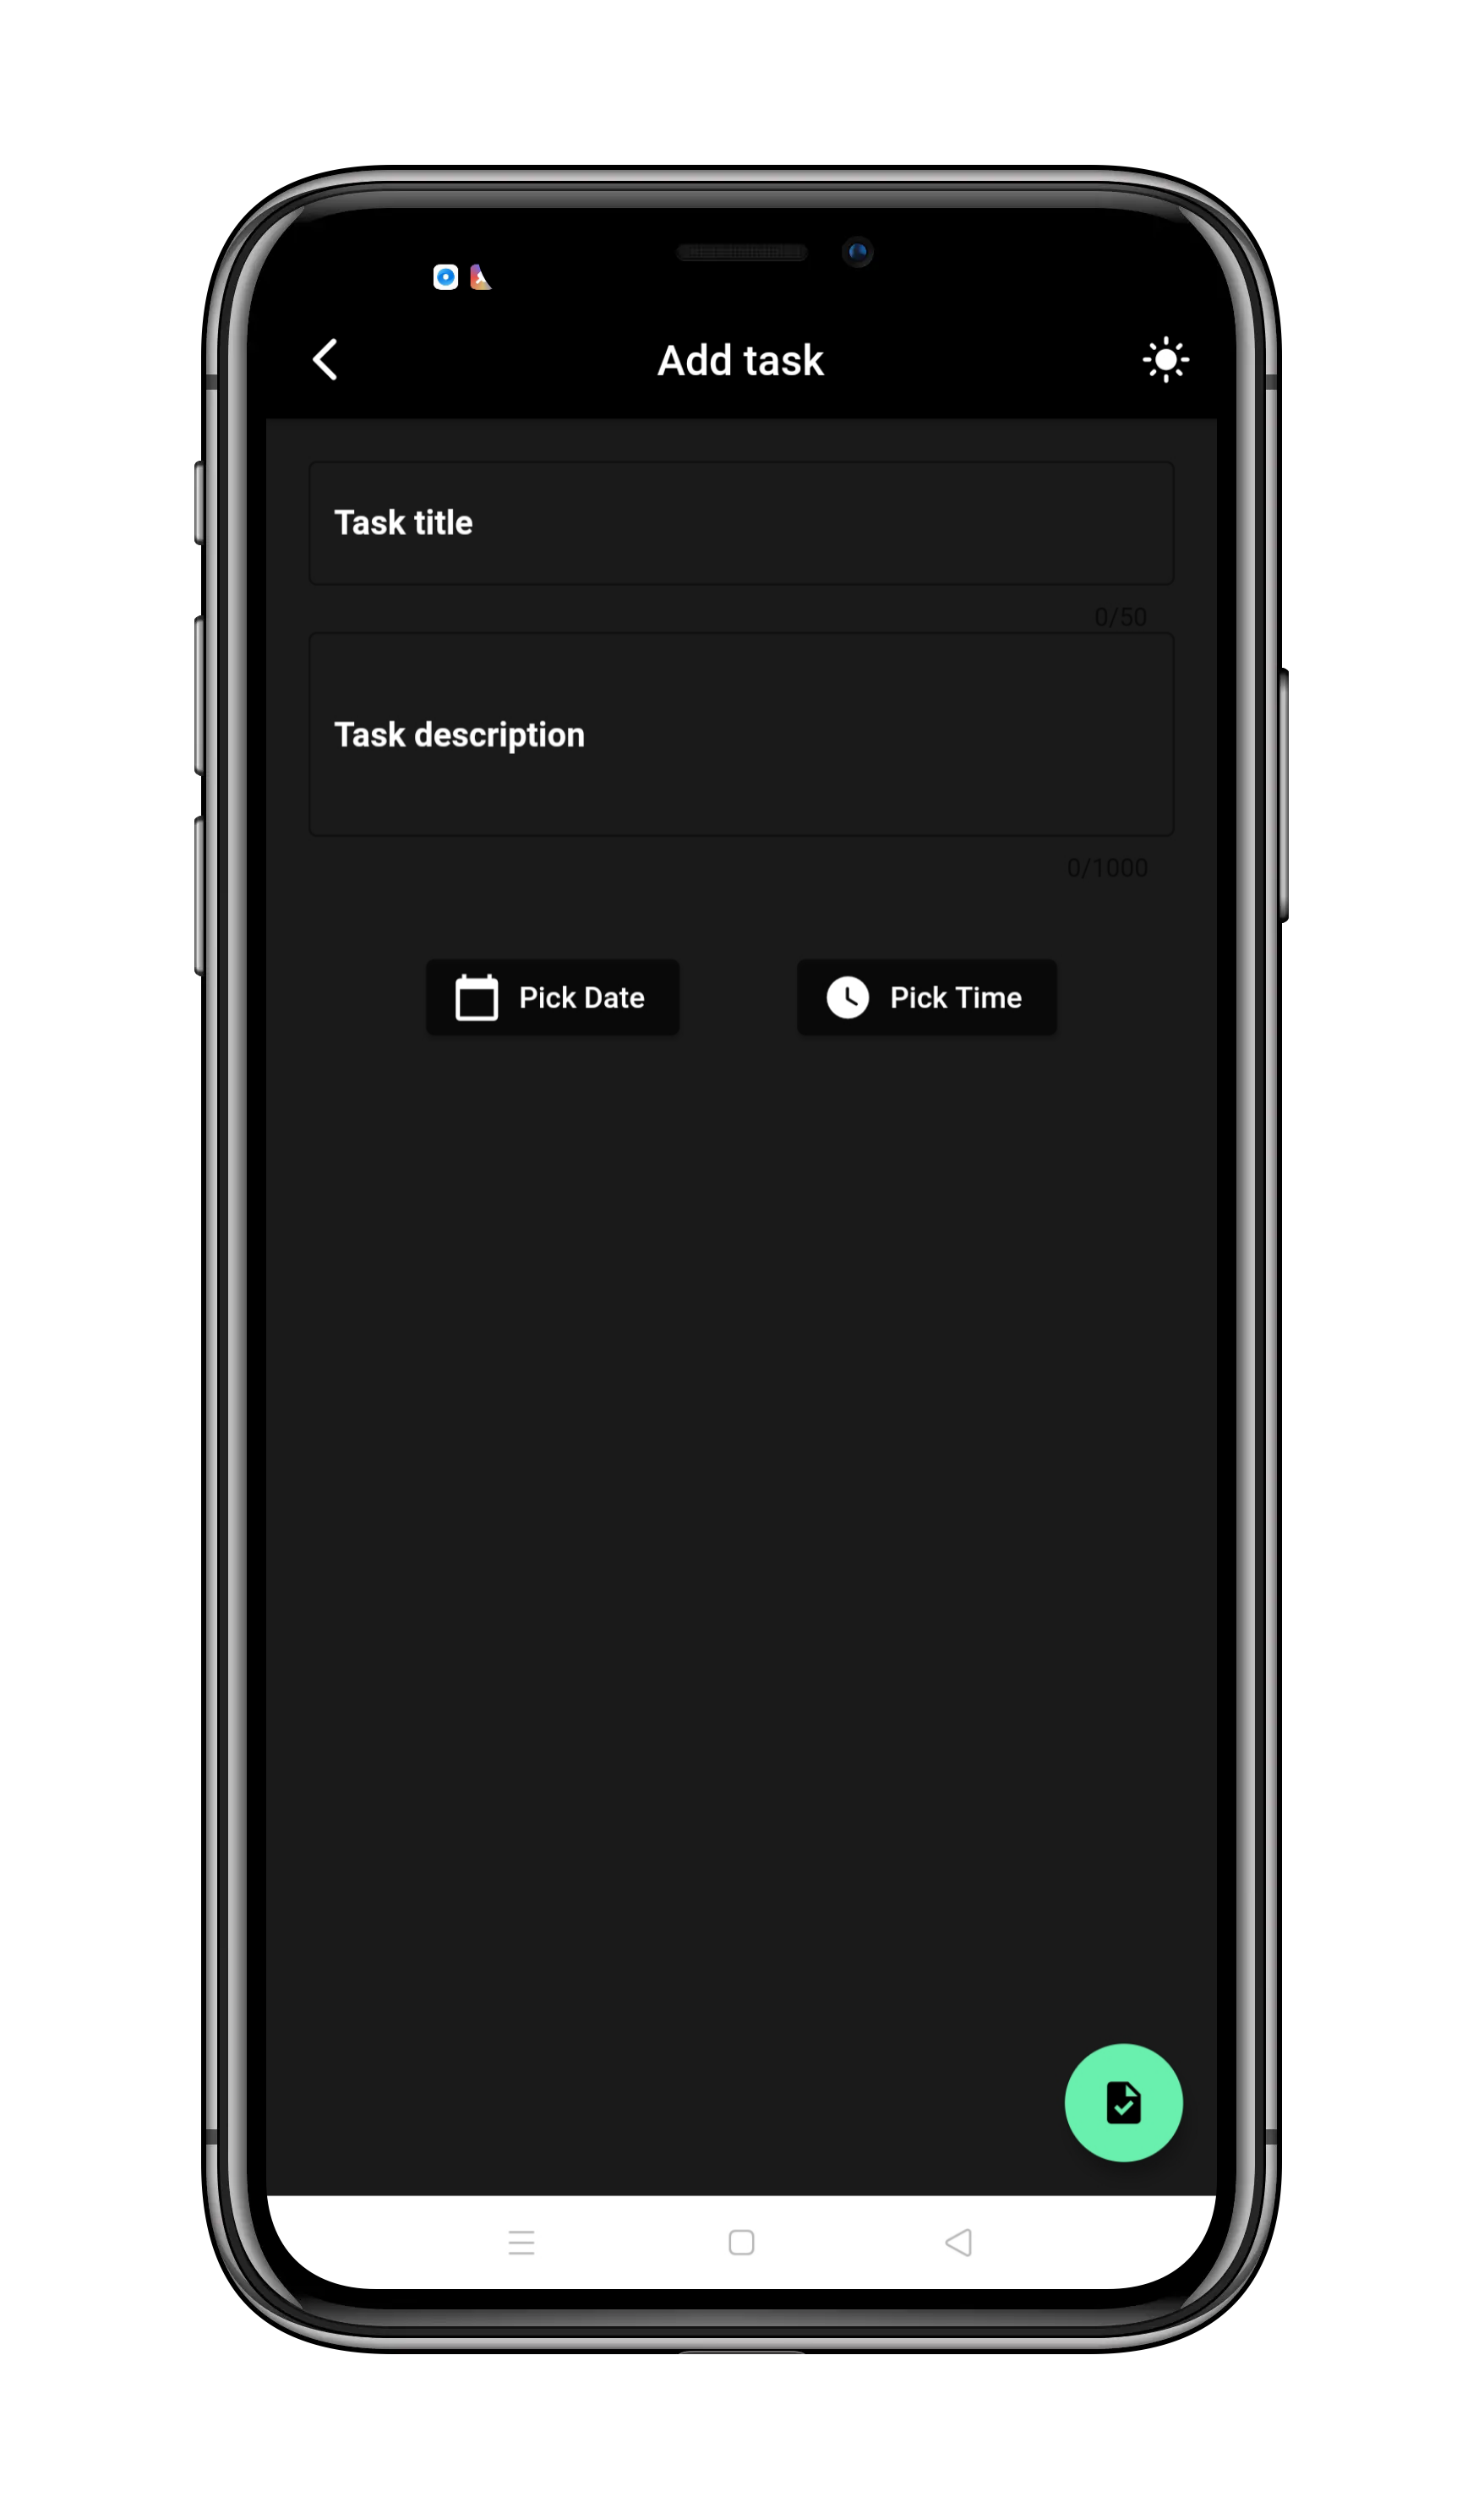
\includegraphics[height=90mm]{Images & Logos/theme/CH_08_Dark_4.png}\\
  \caption{Add Task Page}
\end{minipage}
\newpage
\end{figure}

\begin{figure}[h]
  \begin{center}
   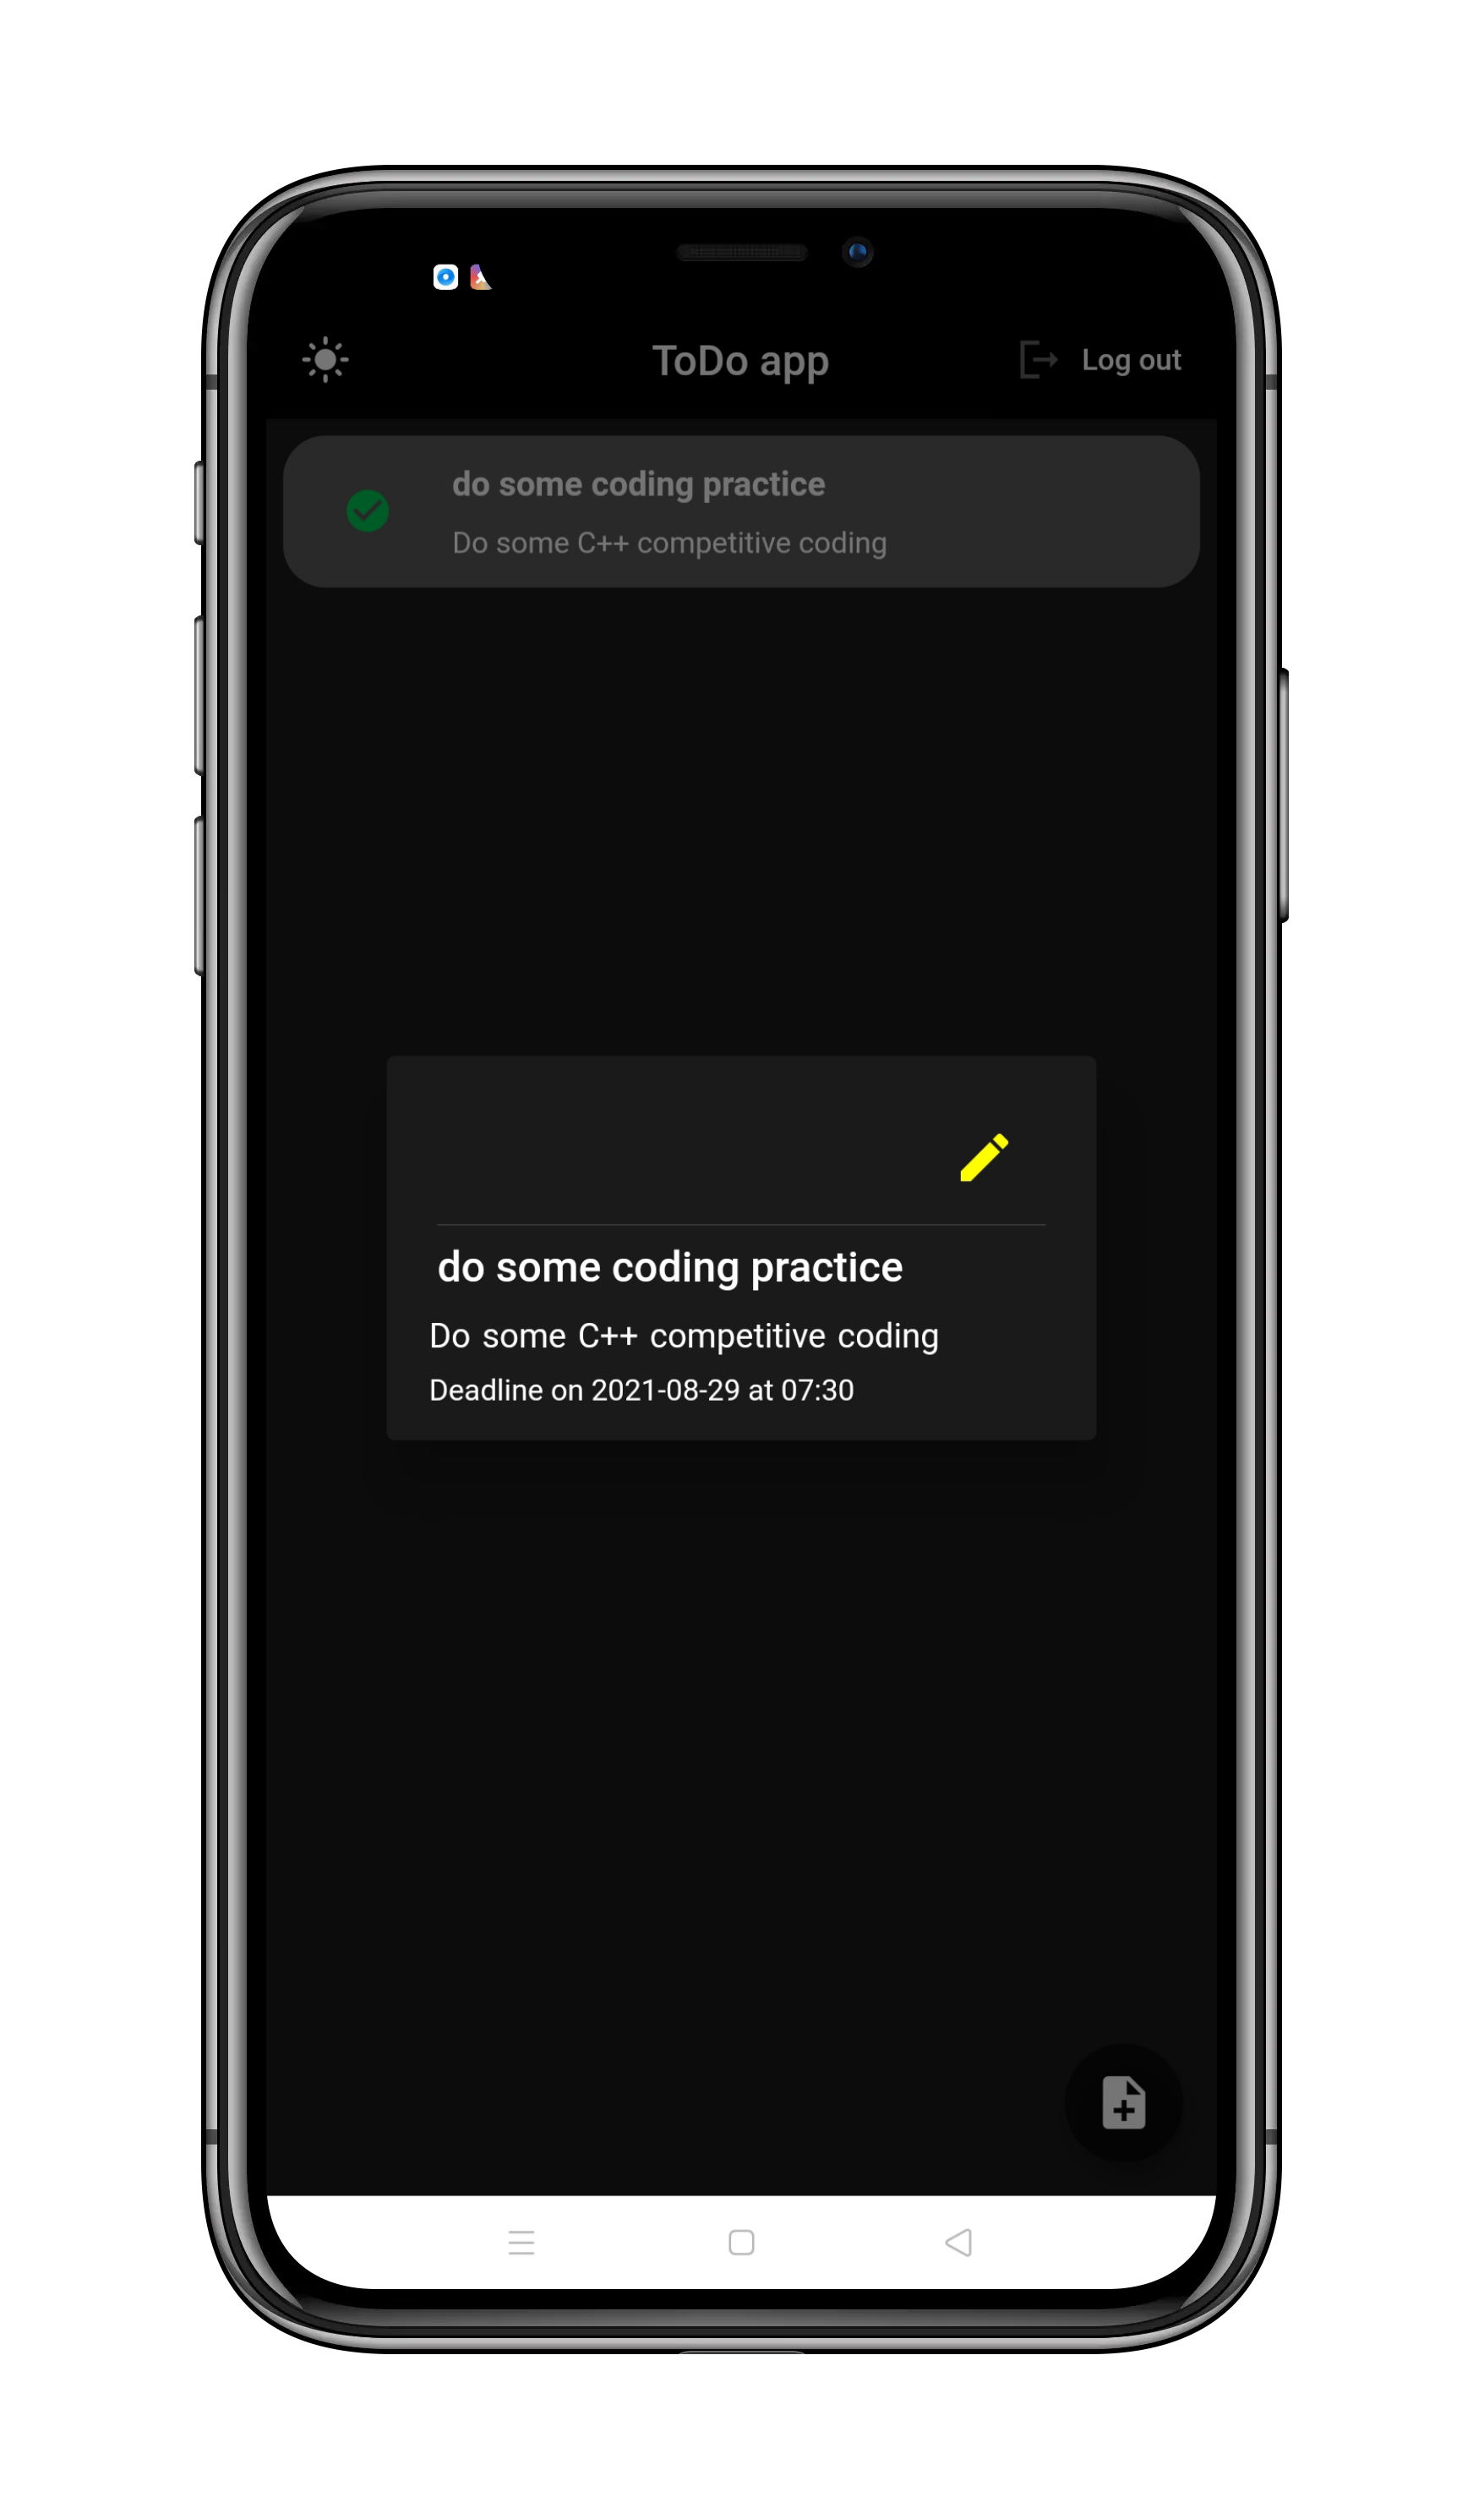
\includegraphics[height=90mm]{Images & Logos/theme/CH_08_Dark_5.png}
%  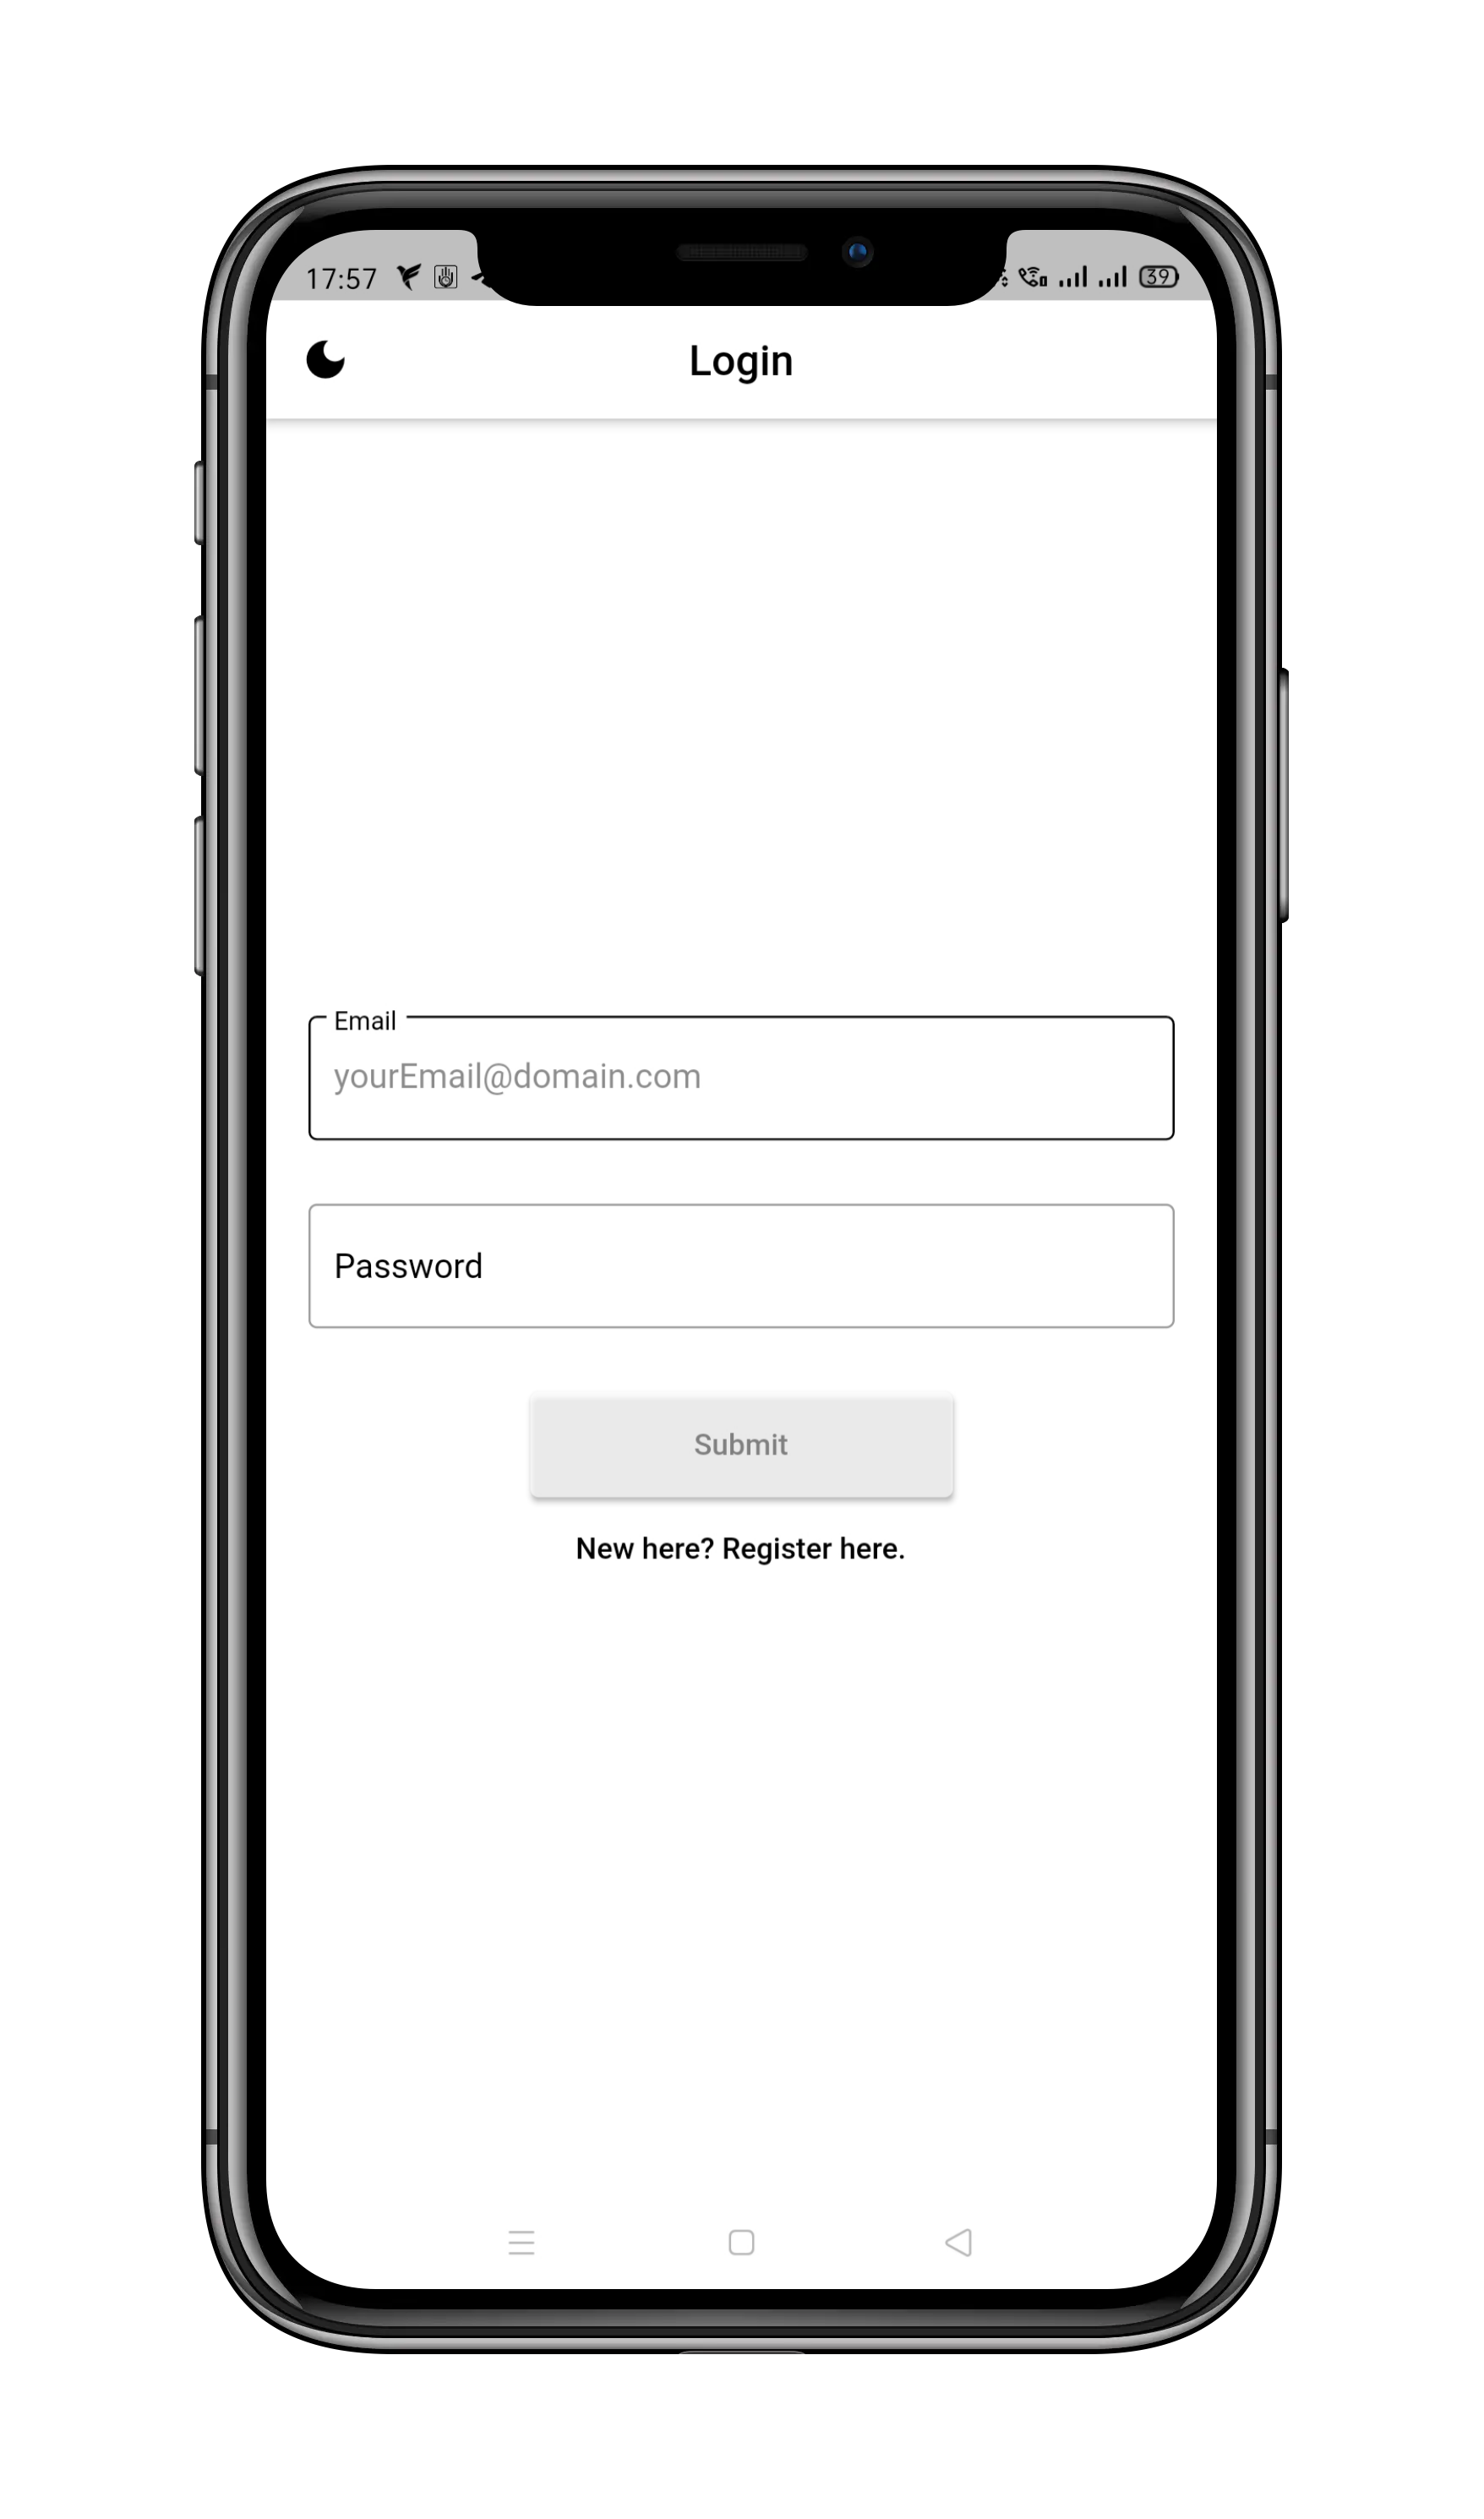
\includegraphics[height=70mm]{Images & Logos/theme/CH_08_Light_1.png}\\
  \end{center}
  \caption{Edit Task Page}
\end{figure}  

.


